\chapter{Method} \label{ch:method}
The subject area of this paper is the registration of scans taken of a large and structurally complex physical objects. In particular the focus is on the registration of long-range scans of the entire Hôtel de Ville building with short-range, high resolution close-up scans of some features of it, like the close-up scan of the dessus-de-porte artwork.

In this chapter a new registration error metric is developed which attempts to make use the point dispersion predictions shown in the previous chapter, in order to improve the registration quality.


\section{Developing an error metric}
Any error metric that does not use the true transformation is an \emph{estimation}, and its global minimum generally does not exactly coincide with the one from the \emph{true error}. But when the true transformation $\matr{M}$ is known, it can be directly compared with the \emph{true error}. An approach to develop a good estimative error metric is the following:
\begin{enumerate} 
\item First the scope is limited to point clouds scans having some \emph{characteristics} that the error metric will make use of.

\item An artificial 3D model which also has these characteristics is defined, along with an algorithm to generate artificial point clouds from it. On these point clouds, the true transformation is known, and parameters such as scanner noise and point errors can be simulated and controlled.

This has been done with the dessus-de-porte scan, and the relief model described in chapter \ref{ch:models}.

\item An estimative error metric is developed that measures the alignment of two different point clouds generated from a model, without taking into account the true transformation $\matr{M}$. It should make use of the said characteristics shared by the model and the real scan.

\item When the estimative error metric works well enough, it is now applied to a real scan. It the artificial point clouds model the real scan well enough, it can be expected to still yield good results. Its accuracy is compared to the \emph{mean absolute error}, and evaluated manually by visual inspection.
\end{enumerate}

In this chapter, an attempt will be made to define a fine registration error metric, based on the histogram formed by the distances of point pairs chosen using the closest point criterion. For this the characteristic dispersion of points on approximatively planar surfaces will be used.


\subsection{High- to low-resolution registration}
The set goal was to improve registration when one point cloud has a lower resolution than the other. Naturally the first step is to develop an error metric which indicates when the point clouds are accurately registered. Then the second step is to develop an algorithm to find a transformation that minimizes this error metric.

This can be considered to be an ill-posed problem when the true transformation $\matr{M}$ is not known: Informally, an error metric attempts to extract information about $\matr{M}$, only from the two input point clouds $P$ and $Q$. When the number of points in $P$ is reduced, there is less information available. Now the goal is to find an algorithm such that $\text{register}(P, Q) = \matr{M}$, based only on the hypothesis that $\matr{M}$ exists. $P$ and $Q$ are data whereas the hypothetical $\matr{M}$ is a physical quantity. In other words it is not well defined what output the algorithm should produce. Point clouds taken from real 3D scans are very unstable data sets to work with because, as indicated in chapter \ref{ch:theory}, both the modeling of the object as a continuous surface and its representation using a set of points are approximations and imply that a degree of uncertainty is associated with every point.

\Gls{icp} with the closest-point criterion essentially relies on the expectation that for all the $q \in Q$, the divergences of a correspondence point $p$ to the true corresponding point $q'$ on the other surface $P$, will cancel each other out because to the large number of points $q$. If the number of points gets lower, this will no longer be the case.

Intuitively, in order to obtain a better error metric, more information about the surfaces needs to be extracted. Standard \gls{icp}'s view of the point cloud $P$ is limited to one corresponding point for each $q \in Q$. As shown in the previous chapter, many variants have been developed that take into account more information, such as the normal vectors, covariance matrices of the error, point attributes, etc.

\subsection{Approach}
Since the scope here is limited to range images, that have near-planar surfaces, the point dispersion pattern that the scanner's rays will produce on the surfaces can be considered to encode information about those surfaces. The following two point clouds are scans from the same object (dessus-de-porte).
\begin{figure}[H]
{
\centering
\setlength{\fboxsep}{0pt}%
\setlength{\fboxrule}{0.5pt}%
\hspace*{\fill}%
\begin{subfigure}{.48\textwidth}
	\fbox{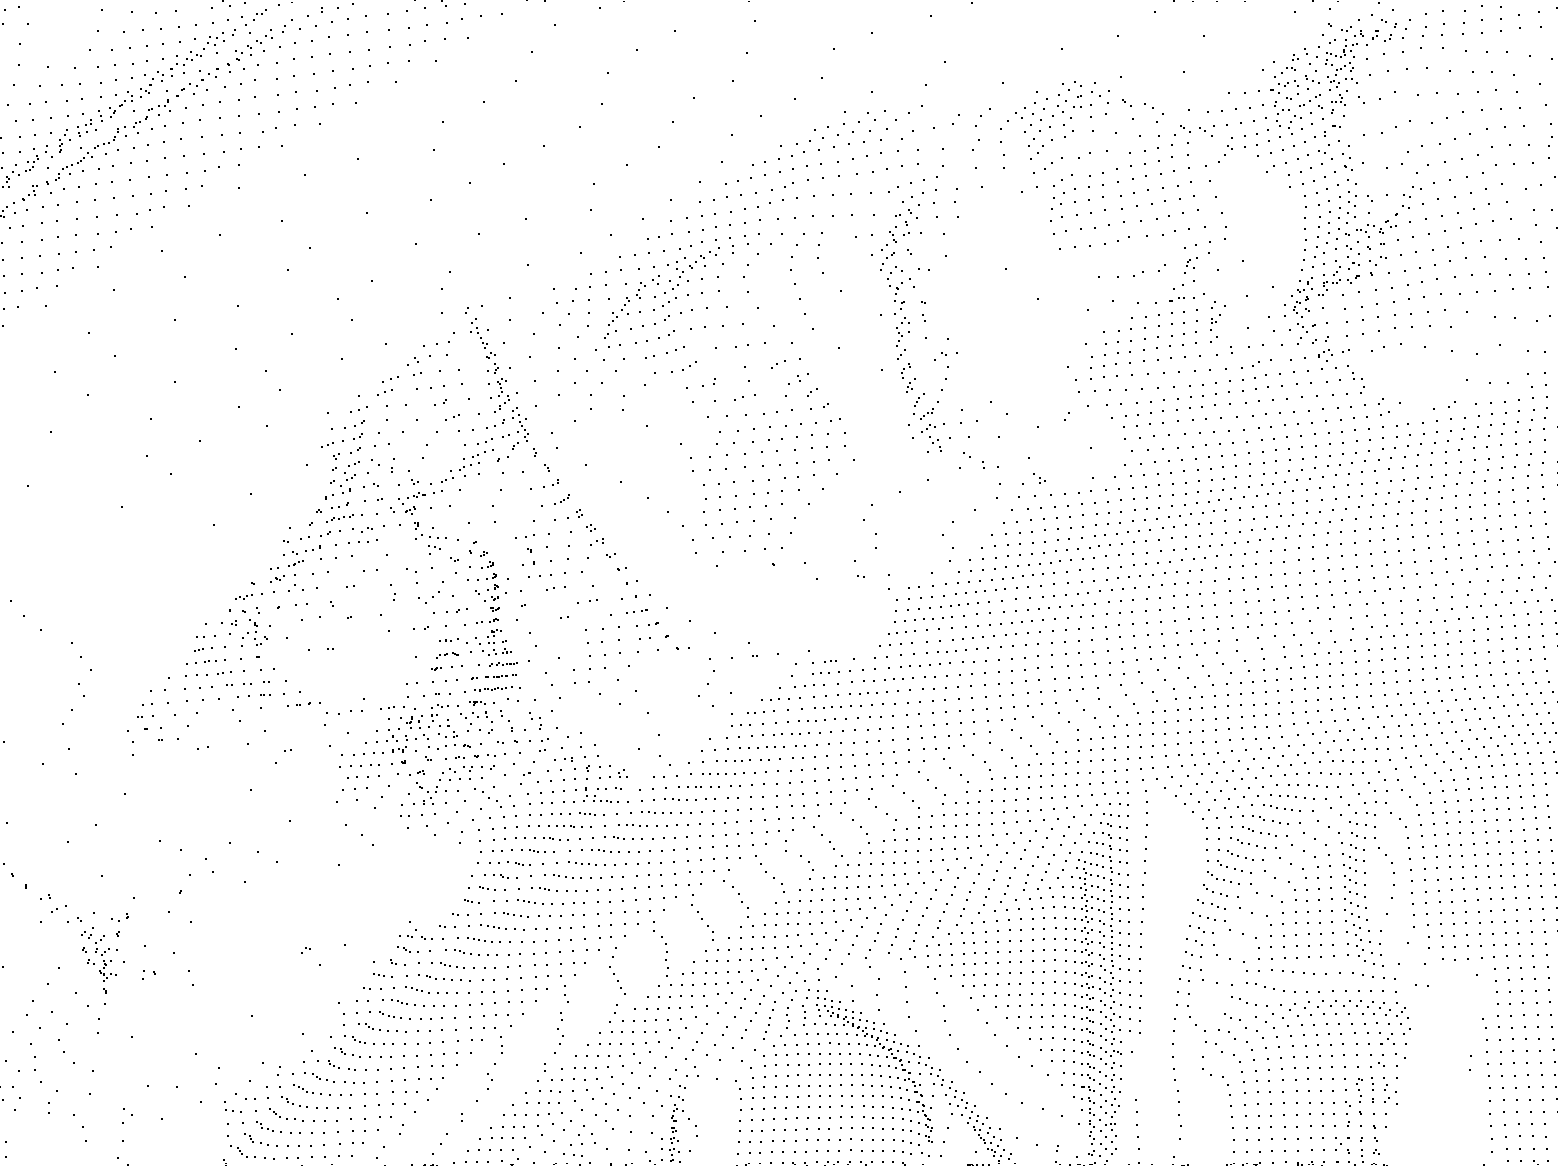
\includegraphics[width=\linewidth]{fig/idea_grid.png}}
	\caption{Points arranged on regular lattice}
\end{subfigure}%
\hfill%
\begin{subfigure}{.48\textwidth}
	\fbox{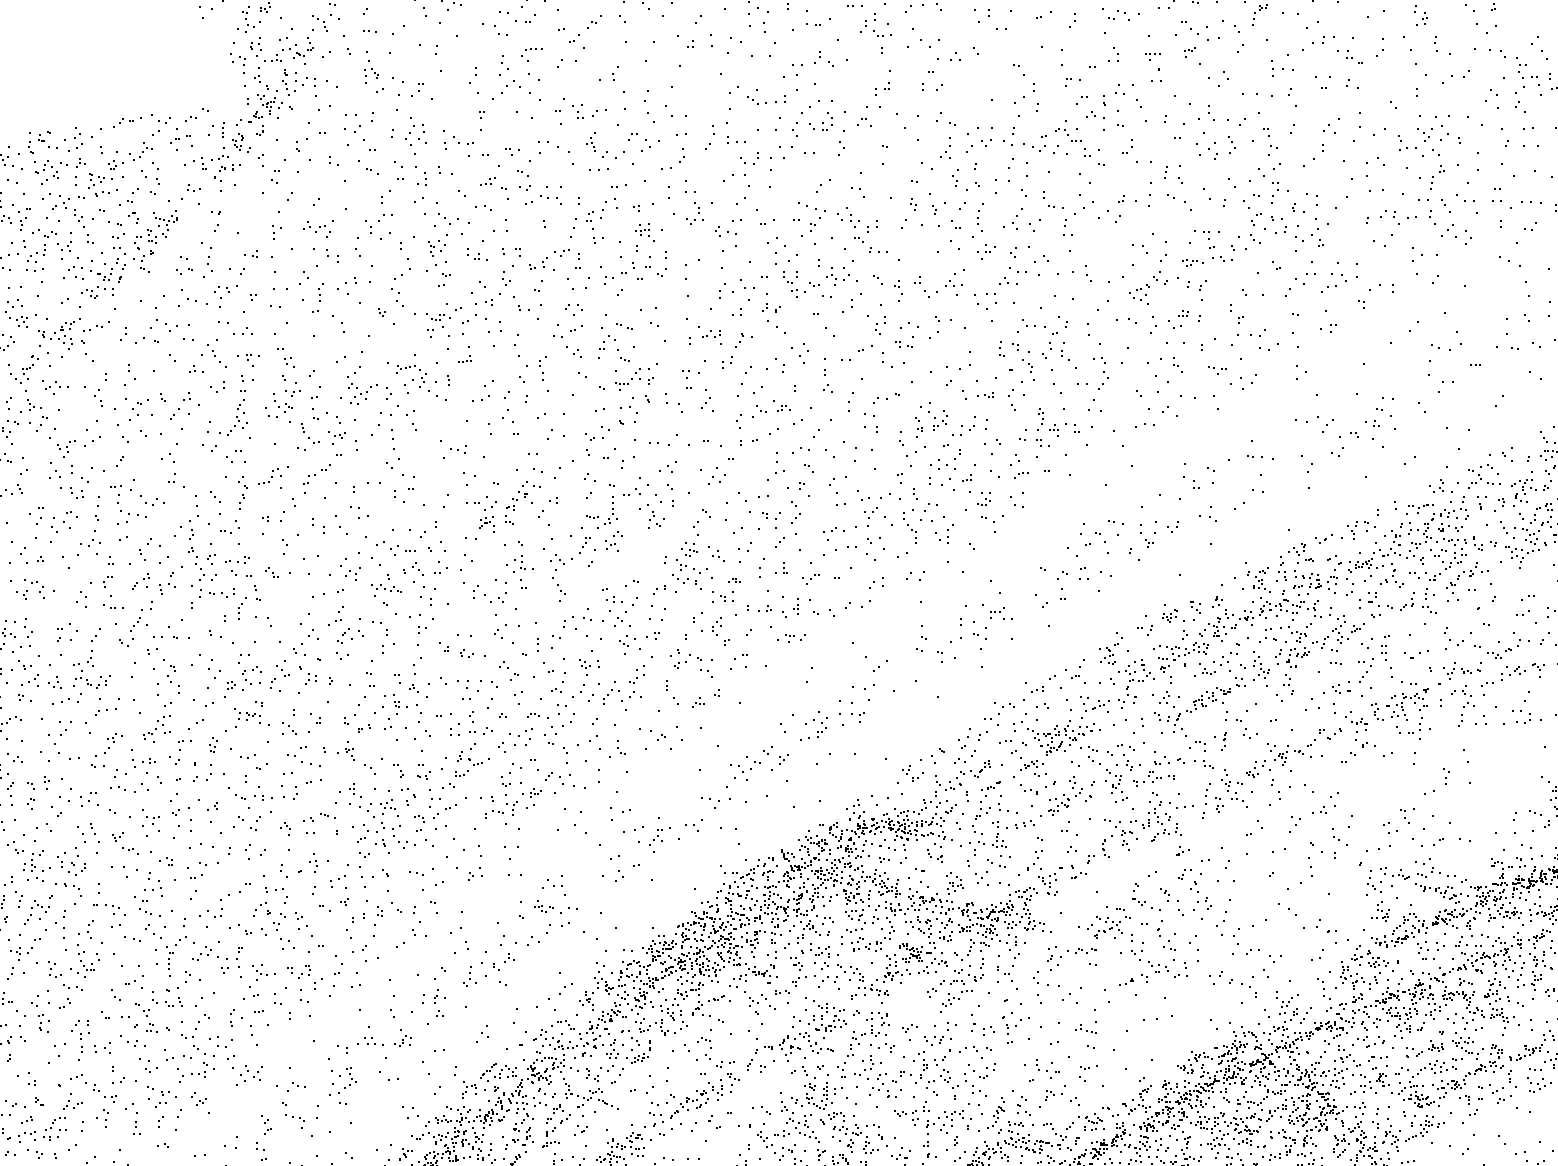
\includegraphics[width=\linewidth]{fig/idea_random.png}}
	\caption{Points dispersed randomly}
\end{subfigure}
}
\caption{Same model, with different point dispersions}
\end{figure}

The first one shows the points' arrangement as produced by the scanner, whereas in the second one they are randomly dispersed, at about the same density.\footnote{It was generated from the higher resolution scan, followed by random downsampling} To a human looking at these two screenshots, is it immediately apparent that the first one contains more information about the object's geometry. To the point-to-point error metric, on the other hand, these two point clouds would ``look'' the same since it does not consider the positions of points in $P$ relative to one another.

The points become arranged so that they form a parallelogram lattice on planar surfaces of the object. When two point clouds $P$ and $Q$ of the same object, from which $Q$ is of higher resolution, are perfectly aligned and superimposed, points $q \in Q$ will fall between adjacent lattice points, and inside the parallelograms that they form.

The algorithm will record all of the distances from $q$ to the closest point $p \in P$ in a histogram. Only points $p$ that lie on locally planar surfaces are considered. At the same time, using the normal vectors of the points $p$ relative to the camera view ray directions, it is possible to predict properties of parallelogram lattice on which $p$ lies. This includes the probability distribution of the distance from any position on the same plane to the closest point of the lattice. This probability density function will be compared to the recorded histogram.

If $P$ and $Q$ are well aligned they should form the same distribution. If not, the distances on the histogram will diverge more because an additional displacement in the third dimension relative to the surface was added. An error metric is deduced from the comparison of the histograms.

Unlike the point-to-point error metric, this looks at the \emph{distribution} of the distances and not just at their \emph{average}. The expected distribution is based on the lattice formed by the points $p \in P$ relative to one another.

\subsection{Outline}
Two error metrics $e_{\chi}(\matr{\hat{M}})$ and $e_{r,\chi}(\matr{\hat{M}})$ will be developed in this chapter. In appendix \ref{sec:chi_err} they will be compared to the \emph{mean absolute error} metric. The following steps will be taken:
\begin{enumerate}
\item First two point clouds $P$ (model) and $Q$ (sample) are considered, which are two perfectly aligned planes. They have different point dispersions, and $Q$ has a higher density than $P$. The histogram of the distances from each $q \in Q$ to its closest point $p \in P$, will be called the \gls{odh}.
\item The shape of the \gls{odh} will be studies depending on the point dispersion on $P$. When $P$ has a parallelogram grid dispersion, the \gls{odh} will feature a linear increase from $0$ to $\frac{1}{2} l_{\text{min}}$. This will be called the histogram's \gls{roi}.
\item Now an \gls{aodh} is constructed whose \gls{roi} always ranges from $0$ to $1$, invariant of $l_{\text{min}}$. For this the estimation of $l_{\text{min}}$ shown in the previous chapter will be used.
\item This \gls{aodh} also has the linear \gls{roi} for approximatively planar point clouds, such as the relief model.
\item Now the \gls{acdh} is considered, which is essentially the same, except that $P$ and $Q$ are no longer perfectly aligned. Some additional constraints are added in choosing correspondences.
\item Its \gls{roi} will become more linear, the better $P$ and $Q$ are aligned. A \emph{chi-square} measurement is used to compare the \gls{acdh} to the expected linearly increasing distribution.
\item This value is the error metric $e_{\chi}(\matr{\hat{M}})$.
\item For $e_{r,\chi}(\matr{\hat{M}})$, points $q$ are first projected onto $P$ using the normal vector of the closest point $p$, and then the same process is repeated, but instead using the distances of the projected points $q'$ to $p$.
\end{enumerate}

\glsreset{odh}
\glsreset{aodh}
\glsreset{roi}
\glsreset{cdh}
\glsreset{acdh}


\newpage


\section{Own distance histogram}
Let $P$ and $Q$ be two perfectly aligned point clouds with identical surfaces, but with different point dispersions. They can differ as described in \ref{sec:registration_robostness}. $P$ is called the \emph{model}, and the points $q \in Q$ the \emph{samples}. For each sample $q \in Q$, the closest point $p \in P$ is chosen, and their distance $\|p - q\|$ is recorded. The histogram of these distances will be called the \gls{odh}. The points $p$ are chosen by the closest point criterion, at first without additional constraints.

In this section the shape of this histogram will be analyzed, and in the next section it will be compared to the \acrfull{cdh}, for which $P$ and $Q$ are no longer identical or perfectly aligned.

By replacing the samples $q \in Q$ with a random variable $\textbf{Q}$ with a given probability distribution, the \gls{odh} can be idealized into a probability density function of the closest point distance, free of noise resulting from the sparse set of samples.

In the following, $Q$ will be taken to have a much higher point density than $P$. When the number of samples becomes infinite, the histogram converges towards the ideal probability density function. The results will later be applied to devise a method for registering high resolution with low resolution point clouds.

When used on two exact same copies of the same point clouds that are perfectly aligned, all measured distances are $0$, and so the histogram consists only of one spike.

When $P$ is artificial and its surface shape is known, $Q$ is constructed by taking a large number of points on that same surface.

\subsection{Plane with random dispersion}
Figure \ref{fig:plane_rand_d30000} shows an \gls{odh}, where $P$ and $Q$ represent a single plane, and the points $p \in P$ are randomly dispersed onto it with an uniform density $\rho(P) = 30000$. For each sample $q$ the distance $d(q, P)$ to the closest point in $P$ is measured. Randomly dispersed means that the $x$ and the $y$ coordinate of each point are chosen randomly and independently, with a uniform distribution in a fixed interval.

Since $P$ and $Q$ are perfectly aligned, in this situation all distances are measured on the two-dimensional plane.

\begin{figure}[H]
\centering
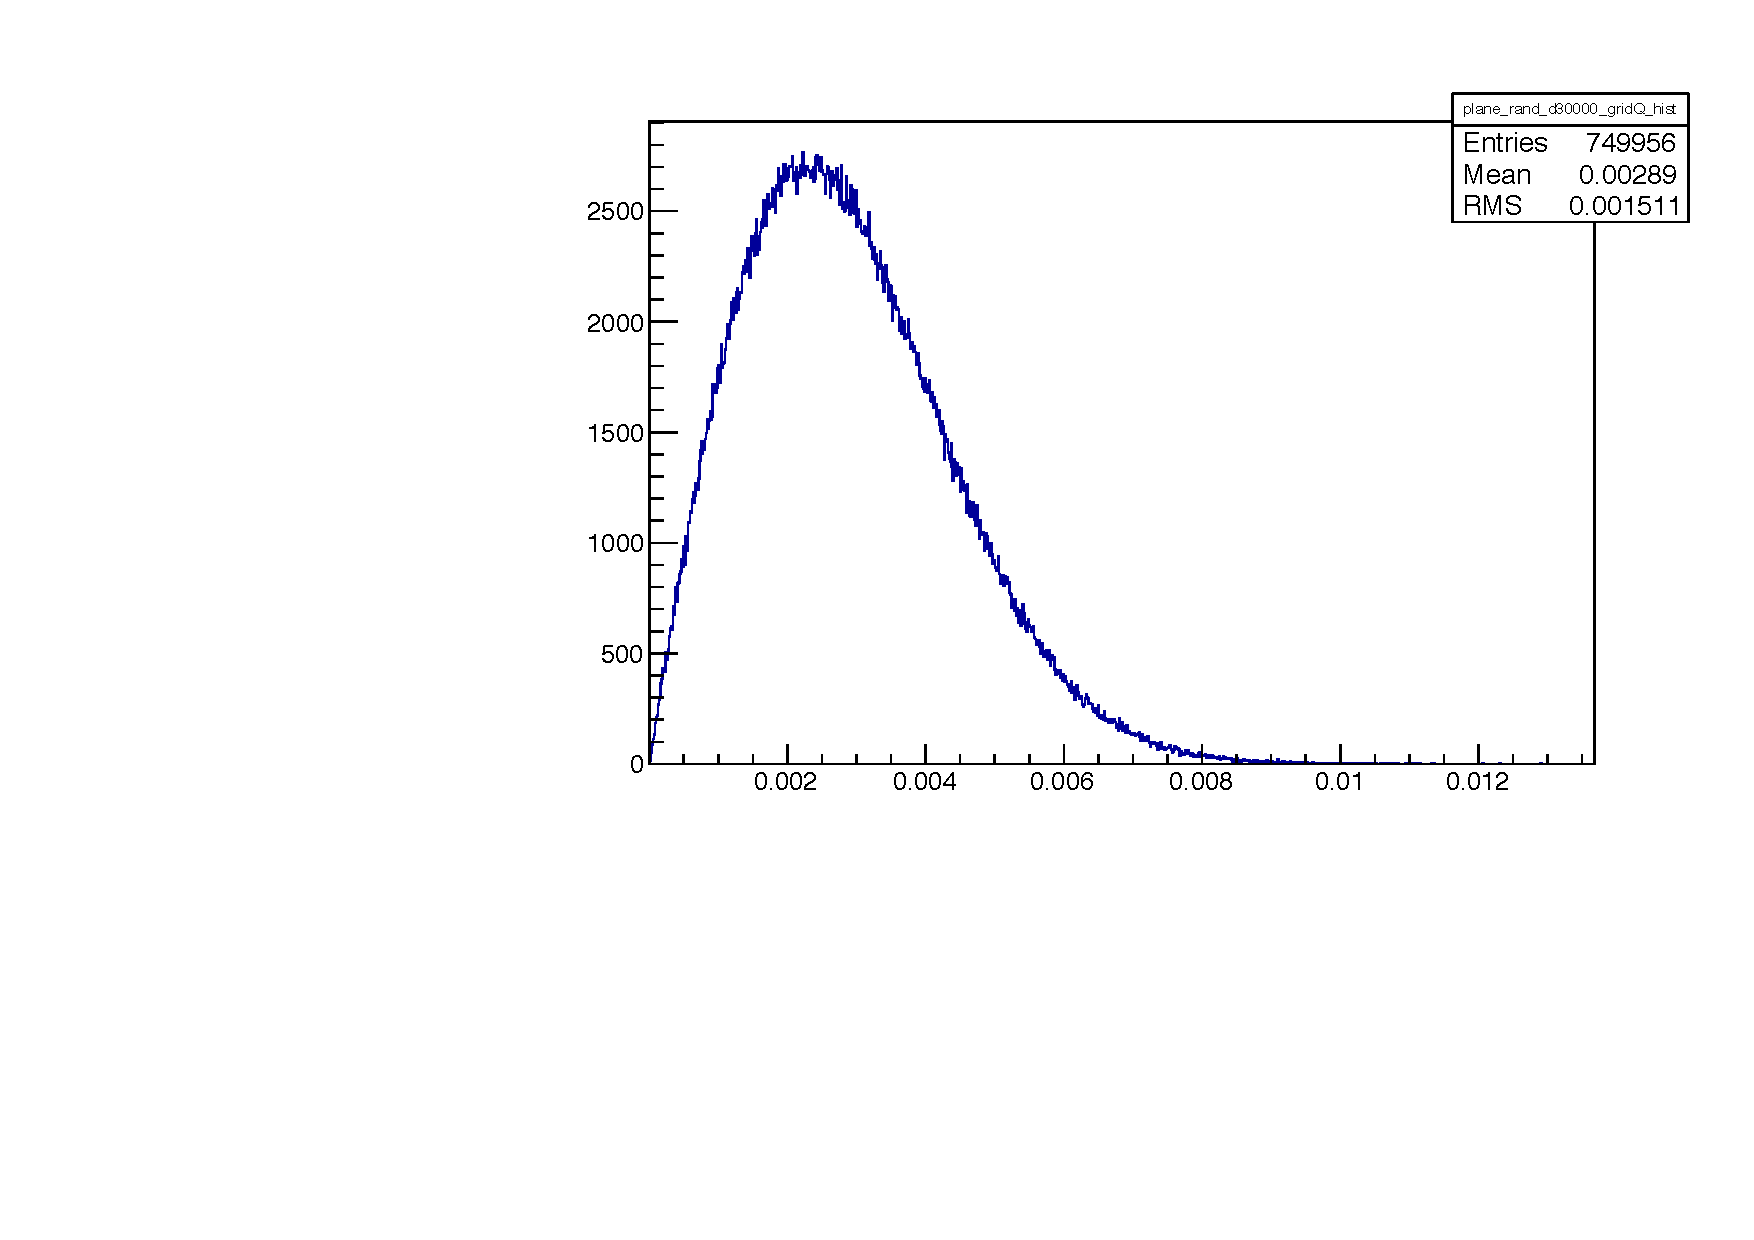
\includegraphics[width=.4\textwidth]{fig/plane_rand_d30000_gridQ.pdf}
\caption{Own distance histogram for plane $P$ with random point distribution}
\label{fig:plane_rand_d30000}
\end{figure}

Unless two points coincide, the probability of $d = 0$ is zero. It then increases, because the probability that a disk with radius $d$ around a sample point $q$ contains at least one $p \in P$ gets larger proportionally to the disk's area. But that disk must not increase in radius to contain more than one point, otherwise the closest distance is the distance to the first, closer point inside the disk, and not its radius. This intuitively explains the global shape of the histogram.

The underlying probability density function $f_R$ of the random closest point distance $R$ from any point $q$ is the exponential function
\begin{equation}
f_R(r) = 2 \pi \rho(P) \, r \, e^{-\pi \rho(P) \, r^2}
\end{equation}
This formula is proven in appendix \ref{sec:proof_rand_disp_plane}. A plot is shown in figure \ref{fig:plane_rand_d}, for $\rho(P) = 30000$. It can be seen that the probability density function takes on the same shape as the histogram. By solving $\frac{\diffd}{\diffd r} f_R(r) = 0$, one obtains that the probability density function reaches its maximum at
\begin{equation}
r_{\text{mode}} = \frac{1}{\sqrt{2 \pi} \sqrt{\rho(P)}}
\end{equation}

The mean $\bar{r}$ value for the closest point distance is obtained using the integral
\begin{equation}
\bar{r} = \int_{0}^{\infty} r \, f_R(r) \, \diffd r = \frac{1}{2 \sqrt{\rho(P)}}
\end{equation}

\begin{figure}[h]
\centering
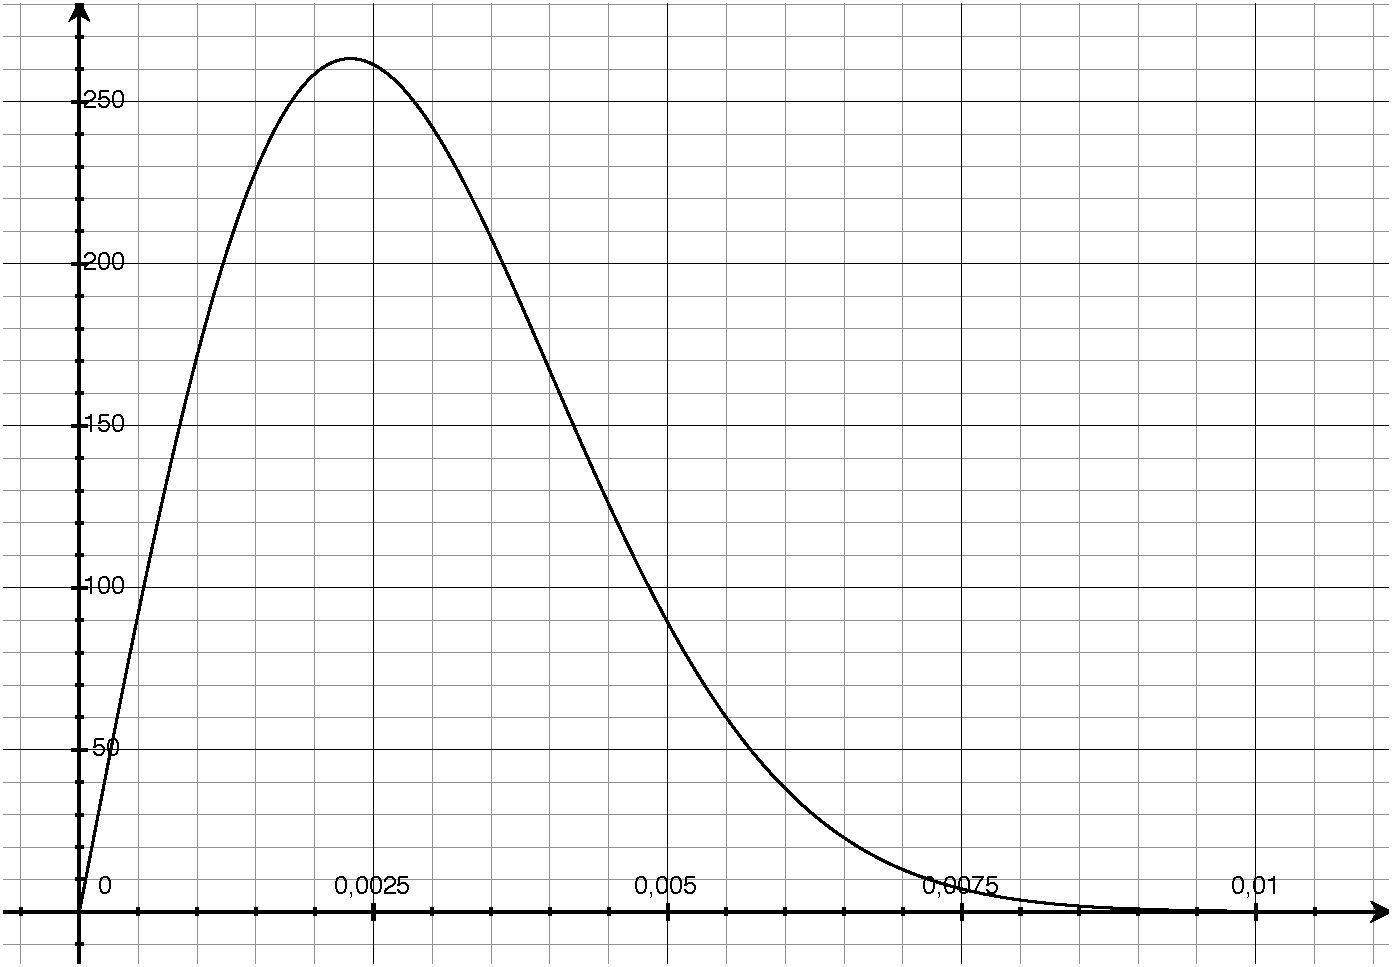
\includegraphics[width=.3\textwidth]{fig/plane_rand_d.pdf}
\caption{Probability density function of closest point distance, for plane $P$ with randomly dispersed points}
\label{fig:plane_rand_d}
\end{figure}

This random points dispersion represents the most general case, where no information about the dispersion of sample points on the surfaces is known. 

\FloatBarrier


\subsection{Dispersion of sample points} \label{sec:disp_sample_pts}
In order to obtain a histogram that closely resembles the theoretical probability density function, the dispersion of the sample points $q \in Q$ should be such that its density is much higher than that of the model points, and has a low variance. If the density is not high enough, the range of possible placements of sample points relative to surrounding model points is sampled too sparsely, leading to a low resolution histogram. If the variance is too high, some placements will be oversampled in comparison to others, and the histogram will contain more noise.

Figure \ref{fig:plane_rand_d30000_randQ} shows the same histogram, but with the sample points $q_i \in Q$ also being randomly dispersed on the plane (and a different number of samples). It is shown in appendix \ref{sec:proof_var_rand_pt_disp} that the local density is not constant.

This effect is greatly reduced when the sample points on $Q$ are instead dispersed on a regular square grid. The deviation of $N(A)$ from $\bar{N}(A)$ then occurs only due to aliasing near the border of the region $A$, so the variance is near-zero. It gets lower with a higher density of the samples $q \in Q$ and consequently lower side length of the square grid. This was used to obtain the histogram \ref{fig:plane_rand_d}.

\begin{figure}[h]
\centering
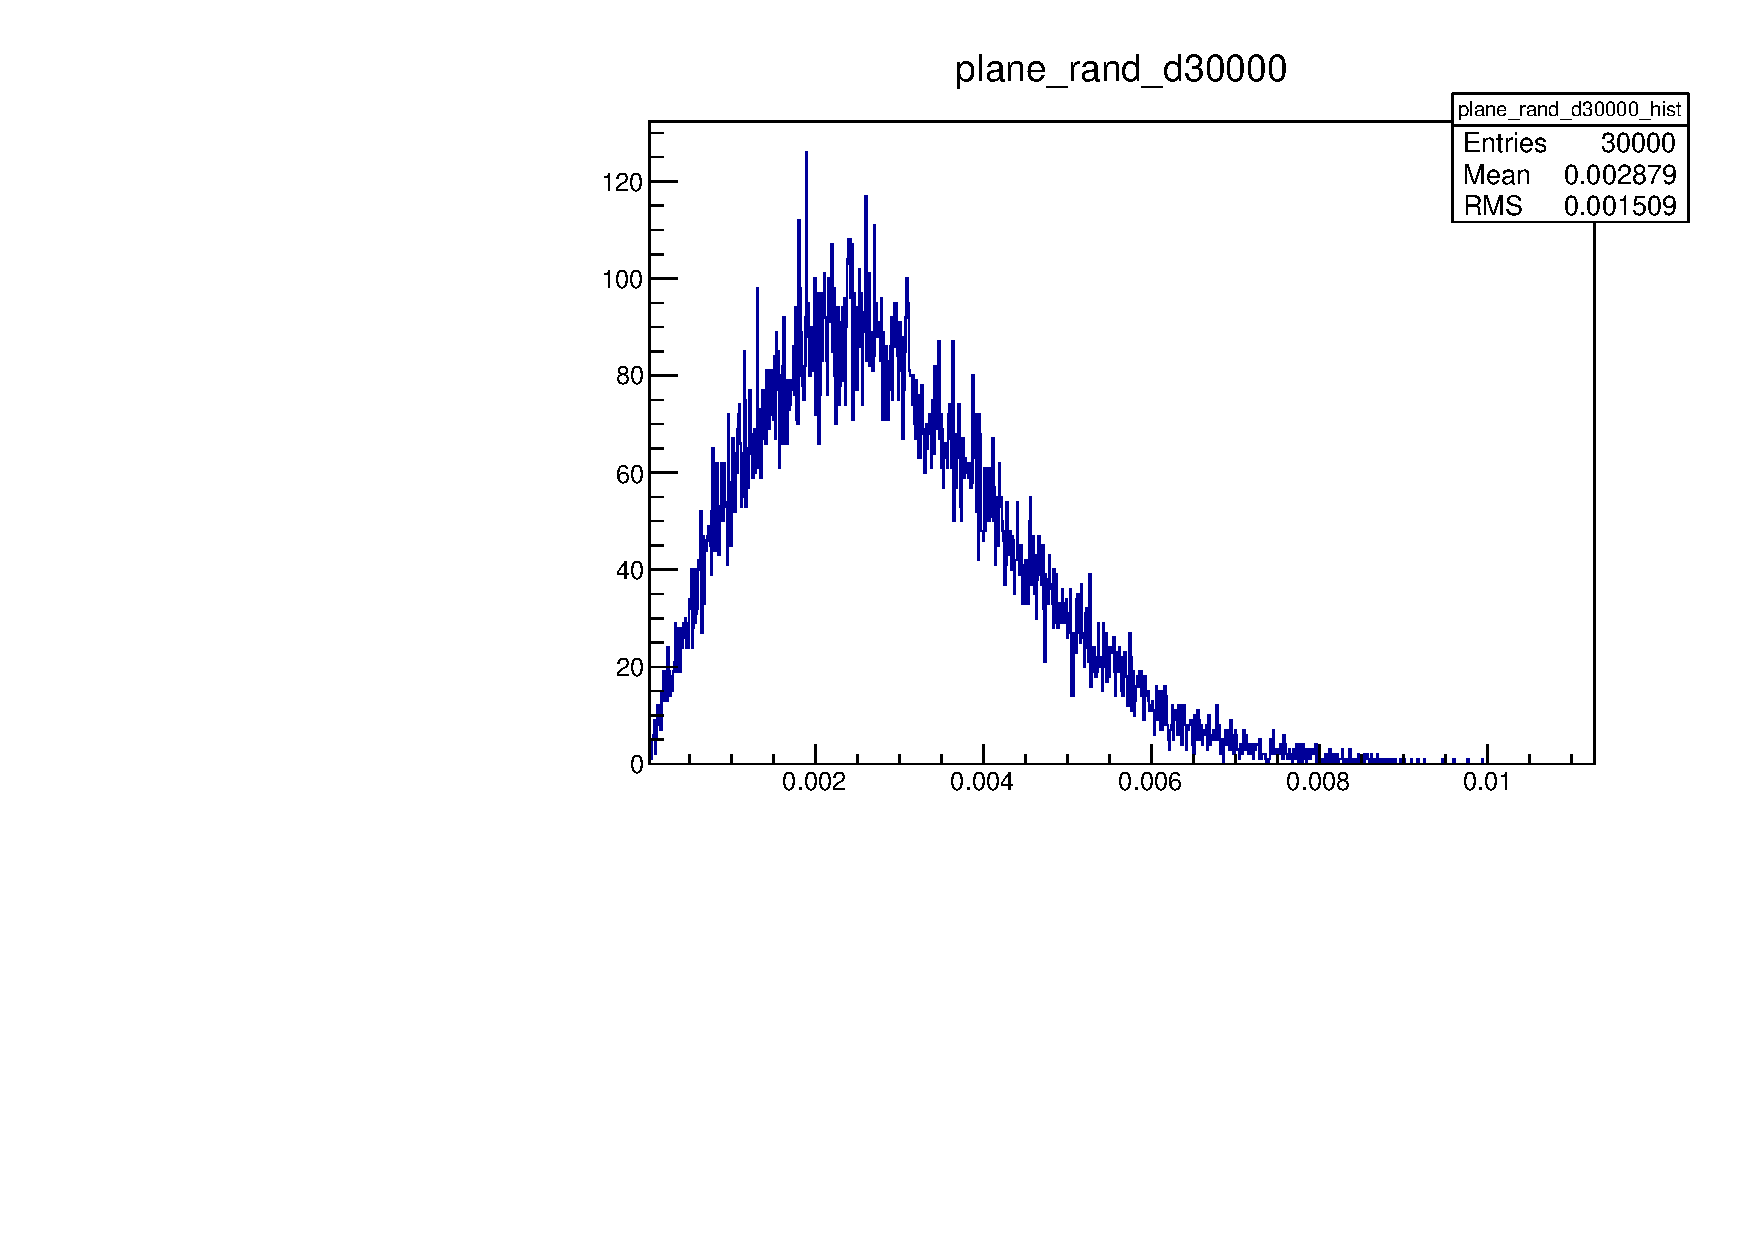
\includegraphics[width=.4\textwidth]{fig/plane_rand_d30000.pdf}
\caption{Same as figure \ref{fig:plane_rand_d30000} but with randomly dispersed samples $q \in Q$}
\label{fig:plane_rand_d30000_randQ}
\end{figure}


When working with artificially generated, perfectly aligned point clouds with a square grid point dispersion, the side lengths $l_P$ and $l_Q$ for the model and the sample point clouds must be chosen such that $\frac{l_P}{l_Q} \notin \mathbb{Q}$, otherwise same placements of sample points relative to model points will repeat, and a larger number of sample points doesn't increase histogram quality. For example if $l_P = 0.1$ and $l_Q = 0.02$, each square of the model will have $25$ sample points placed within it at the same relative positions. Taking into account that floating point numbers with limited precision are used, it means that when considering $l_P$ and $l_Q$ to be rational numbers, they should be chosen such that their least common multiple is as high as possible.


\subsection{Plane with square grid dispersion}
Figure \ref{fig:plane_cphist} shows the distance histogram of two perfectly aligned planar surfaces $P$ and $Q$, where the points on $P$ are dispersed on a square grid. $\rho(P) = 20000$ and $30000$, respectively. The number of samples is $N(Q) = 300000$.

\begin{figure}[H]
\centering
\hspace*{\fill}%
\begin{subfigure}{.4\textwidth}
	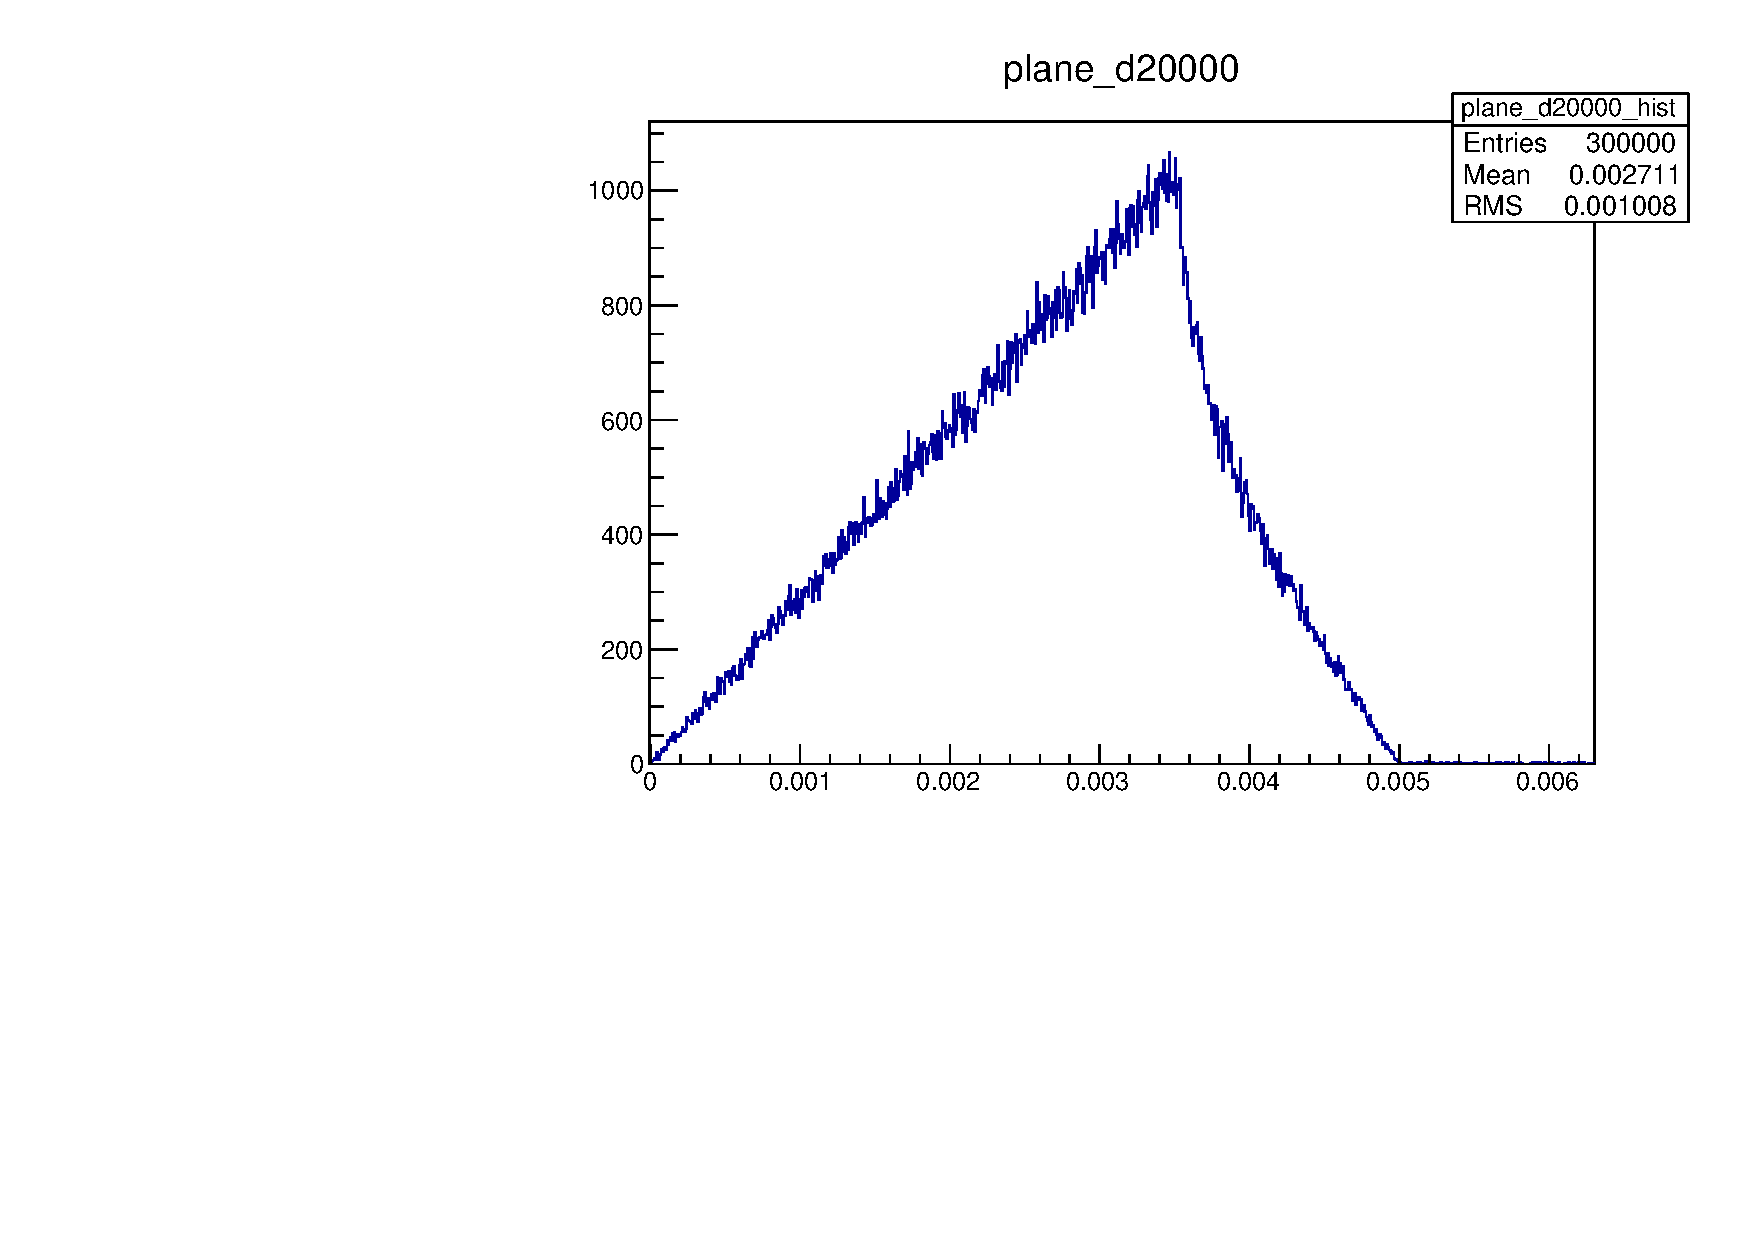
\includegraphics[width=\linewidth]{fig/plane_d20000.pdf}
\end{subfigure}%
\hfill{}%
\begin{subfigure}{.4\textwidth}
	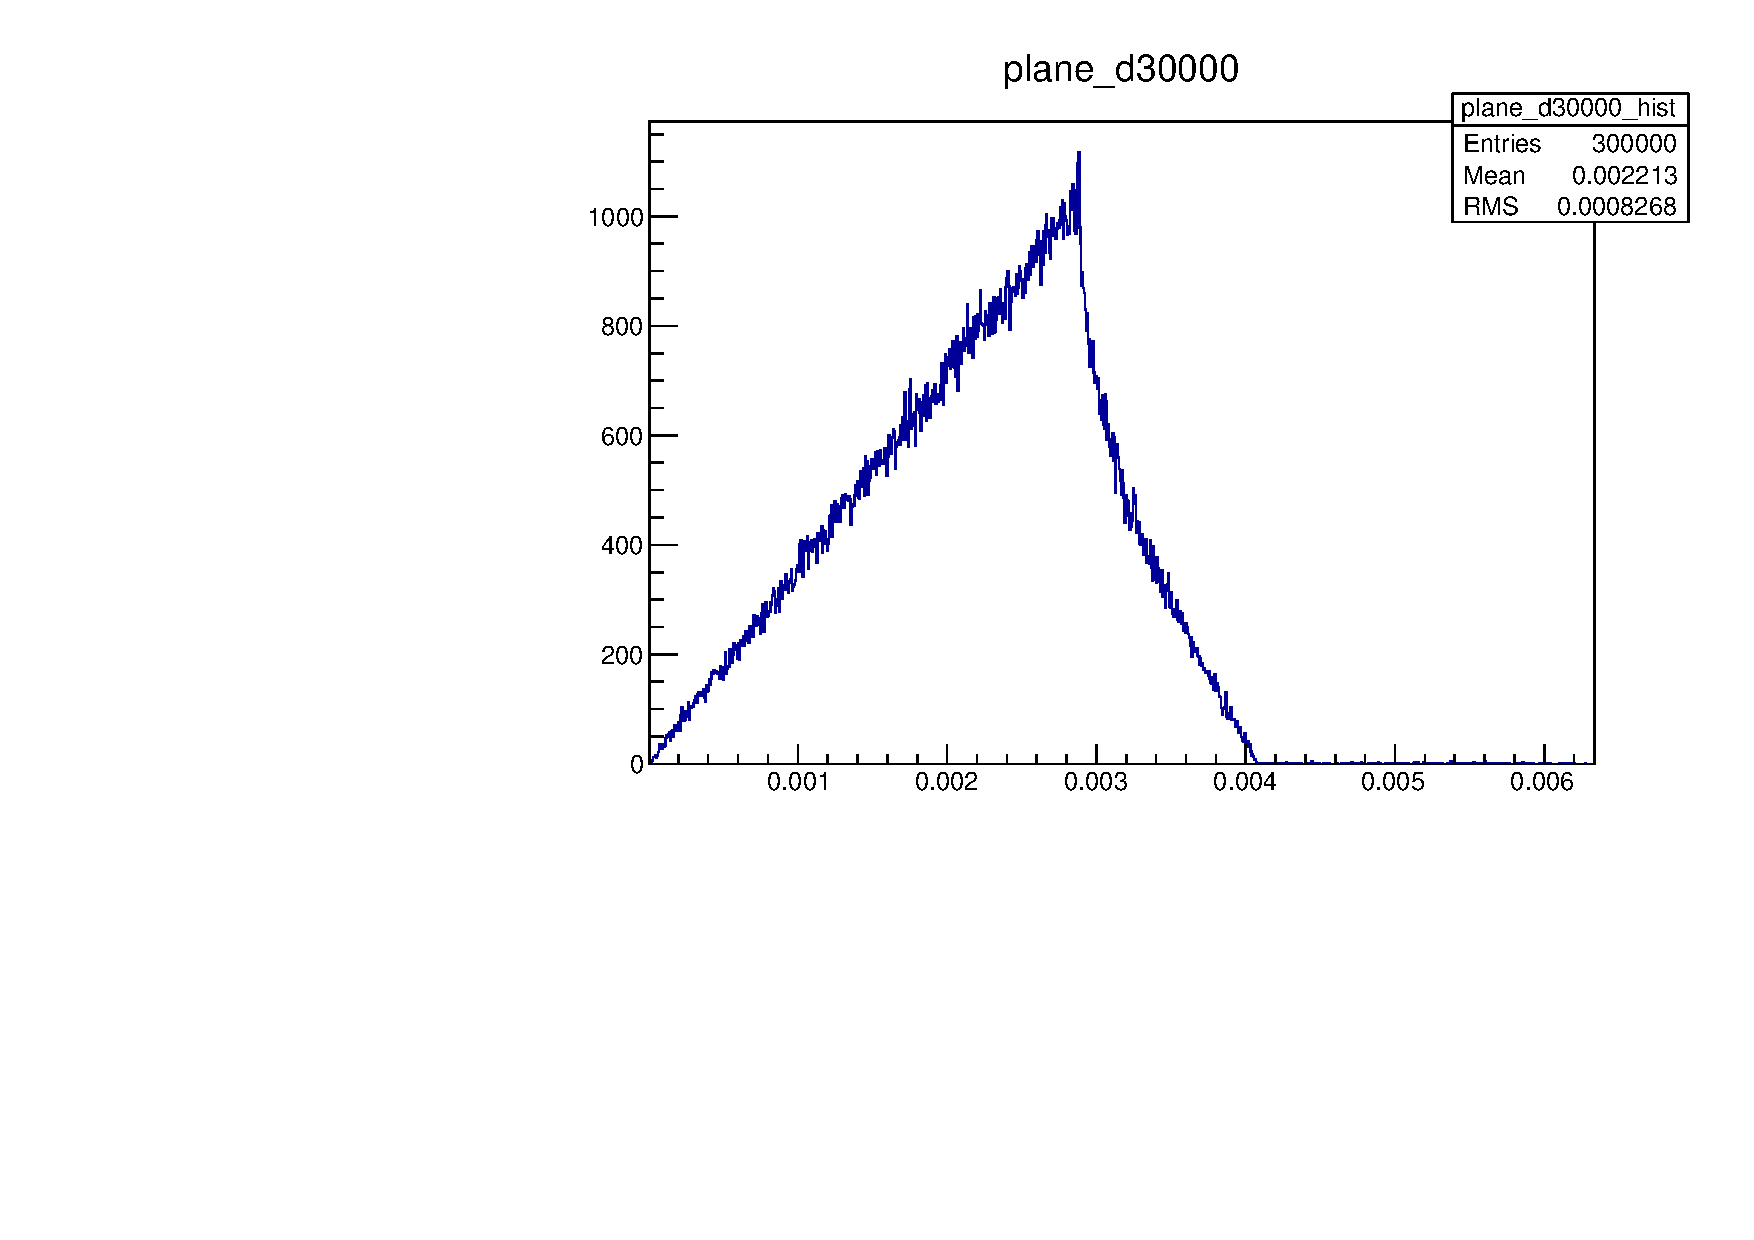
\includegraphics[width=\linewidth]{fig/plane_d30000.pdf}
\end{subfigure}%
\hspace*{\fill}
\caption{Own distance histogram for plane $P$ with square grid point dispersion}
\label{fig:plane_cphist}
\end{figure}

The probability density function $f_R$ is
\begin{equation}
f_R(r) = \frac{r}{2 l} \times \begin{cases}
	\frac{\pi}{4} & 0 \leq r \leq \frac{l}{2} \\
	\frac{\pi}{4} - \arctan{\sqrt{\left( \frac{2r}{l} \right)^2 - 1}} & \frac{l}{2} < r < \frac{l}{2} \sqrt{2}
\end{cases}
\end{equation}
with $l = \frac{1}{\sqrt{\rho(P)}}$. This is proven in appendix \ref{sec:proof_sqgrid_disp_plane}. The plot is shown in figure \ref{fig:sq_grid_d} for $l = 2$.

The probability rises linearily from $O$ to to its mode at $r = \frac{l}{2}$. Within that range, the sample point falls within the non-overlapping disks of radius $\frac{l}{2}$ around the model points.

\begin{figure}[h]
\centering
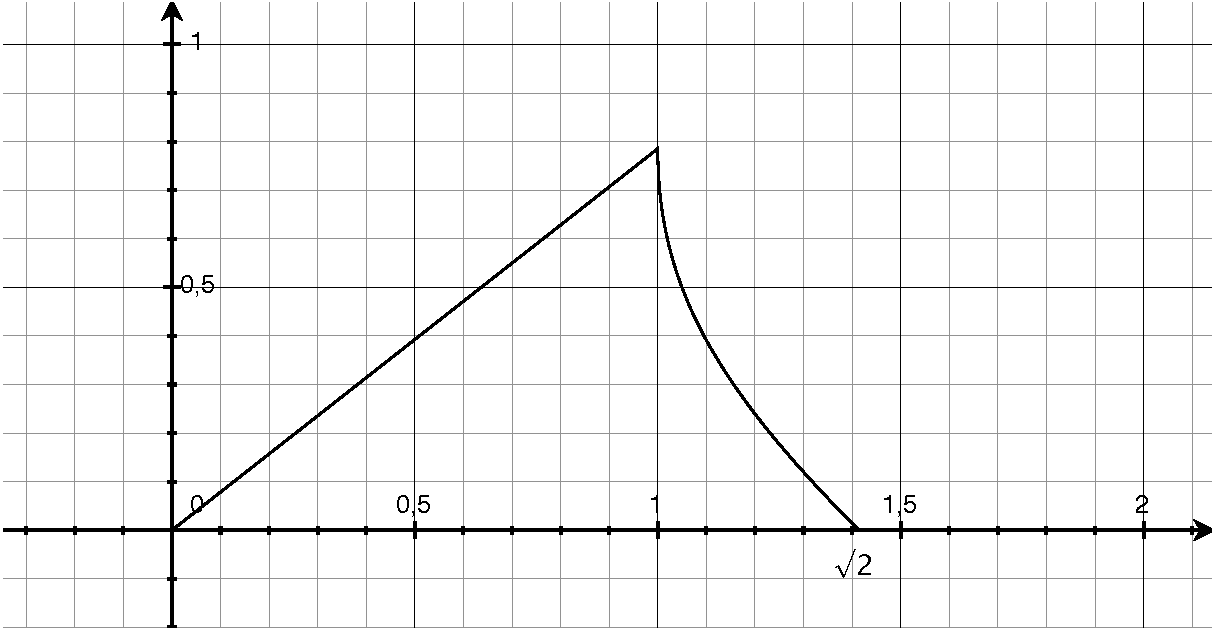
\includegraphics[width=.3\textwidth]{fig/sq_grid_d.pdf}
\caption{Probability density function of closest point distance, for plane $P$ with square grid point arrangement}
\label{fig:sq_grid_d}
\end{figure}

\FloatBarrier

\subsection{Plane with parallelogram grid dispersion}
The square grid dispersion in a special case of the parallelogram grid dispersion. Figure \ref{fig:plane_par_cphist} shows an example of an own closest point histogram obtained when the model point cloud has a parallelogram grid point dispersion. As seen on figure \ref{fig:pargrid_proj}, it is the result of a parallel projection of a square grid on the camera image frame onto a plane in space with a normal vector $\vec{n}$, relative to the camera's coordinate system. For this example, $\vec{n} \approx \transpose{(-0.253023, 0.787174, -0.562438)}$, and the square grid on the image plane has a side length of $p_l = 0.067$.

Figure \ref{fig:par_grid} is a close-up view of the plane, showing the parallelogram grid of $P$, and the higher density square grid sample point cloud $Q$ in blue.


\begin{figure}[H]
\centering
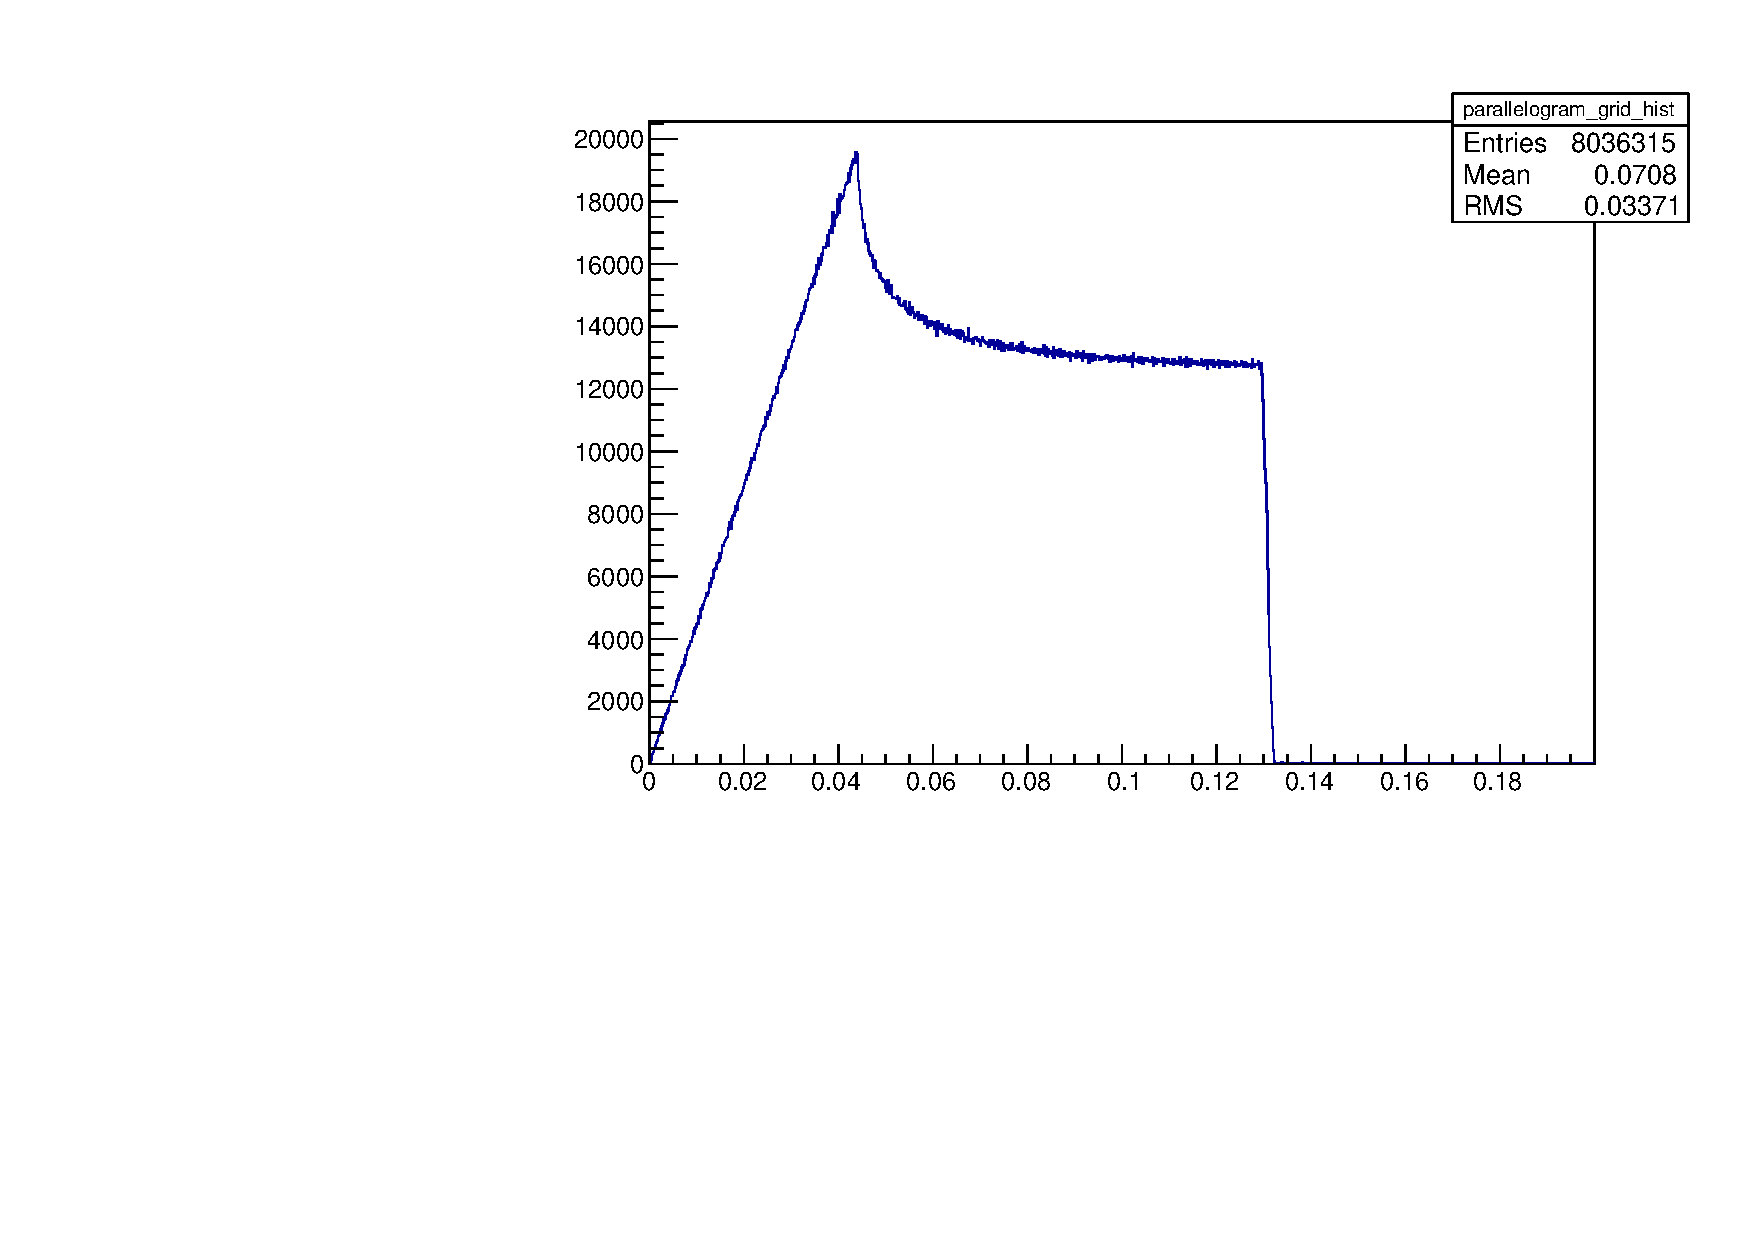
\includegraphics[width=.4\textwidth]{fig/parallelogram_grid.pdf}
\caption{\gls{Gls} for plane $P$ with parallelogram grid point dispersion}
\label{fig:plane_par_cphist}
\end{figure}

It can be seen that the histogram's underlying probability density function is again a piecewise function, and that its first segment is still a linear increase from the zero point up to the mode of the histogram.

Using a similar argument as for the square grid dispersion, one can show that the linear increase happens from $0$ to $\frac{1}{2} l_\text{min}$. Applying the formula \ref{eq:pargrid_lmin} developed in the previous section, a value of approximatively $0.0441$ is found for this example. It corresponds to the mode seen on the histogram.

This segment of linear increase will be called the \acrfull{roi} of the histogram. It will be used to construct an error metric.

\begin{figure}[h]
\centering
{
	\setlength{\fboxsep}{0pt}%
	\setlength{\fboxrule}{0.5pt}%
	\fbox{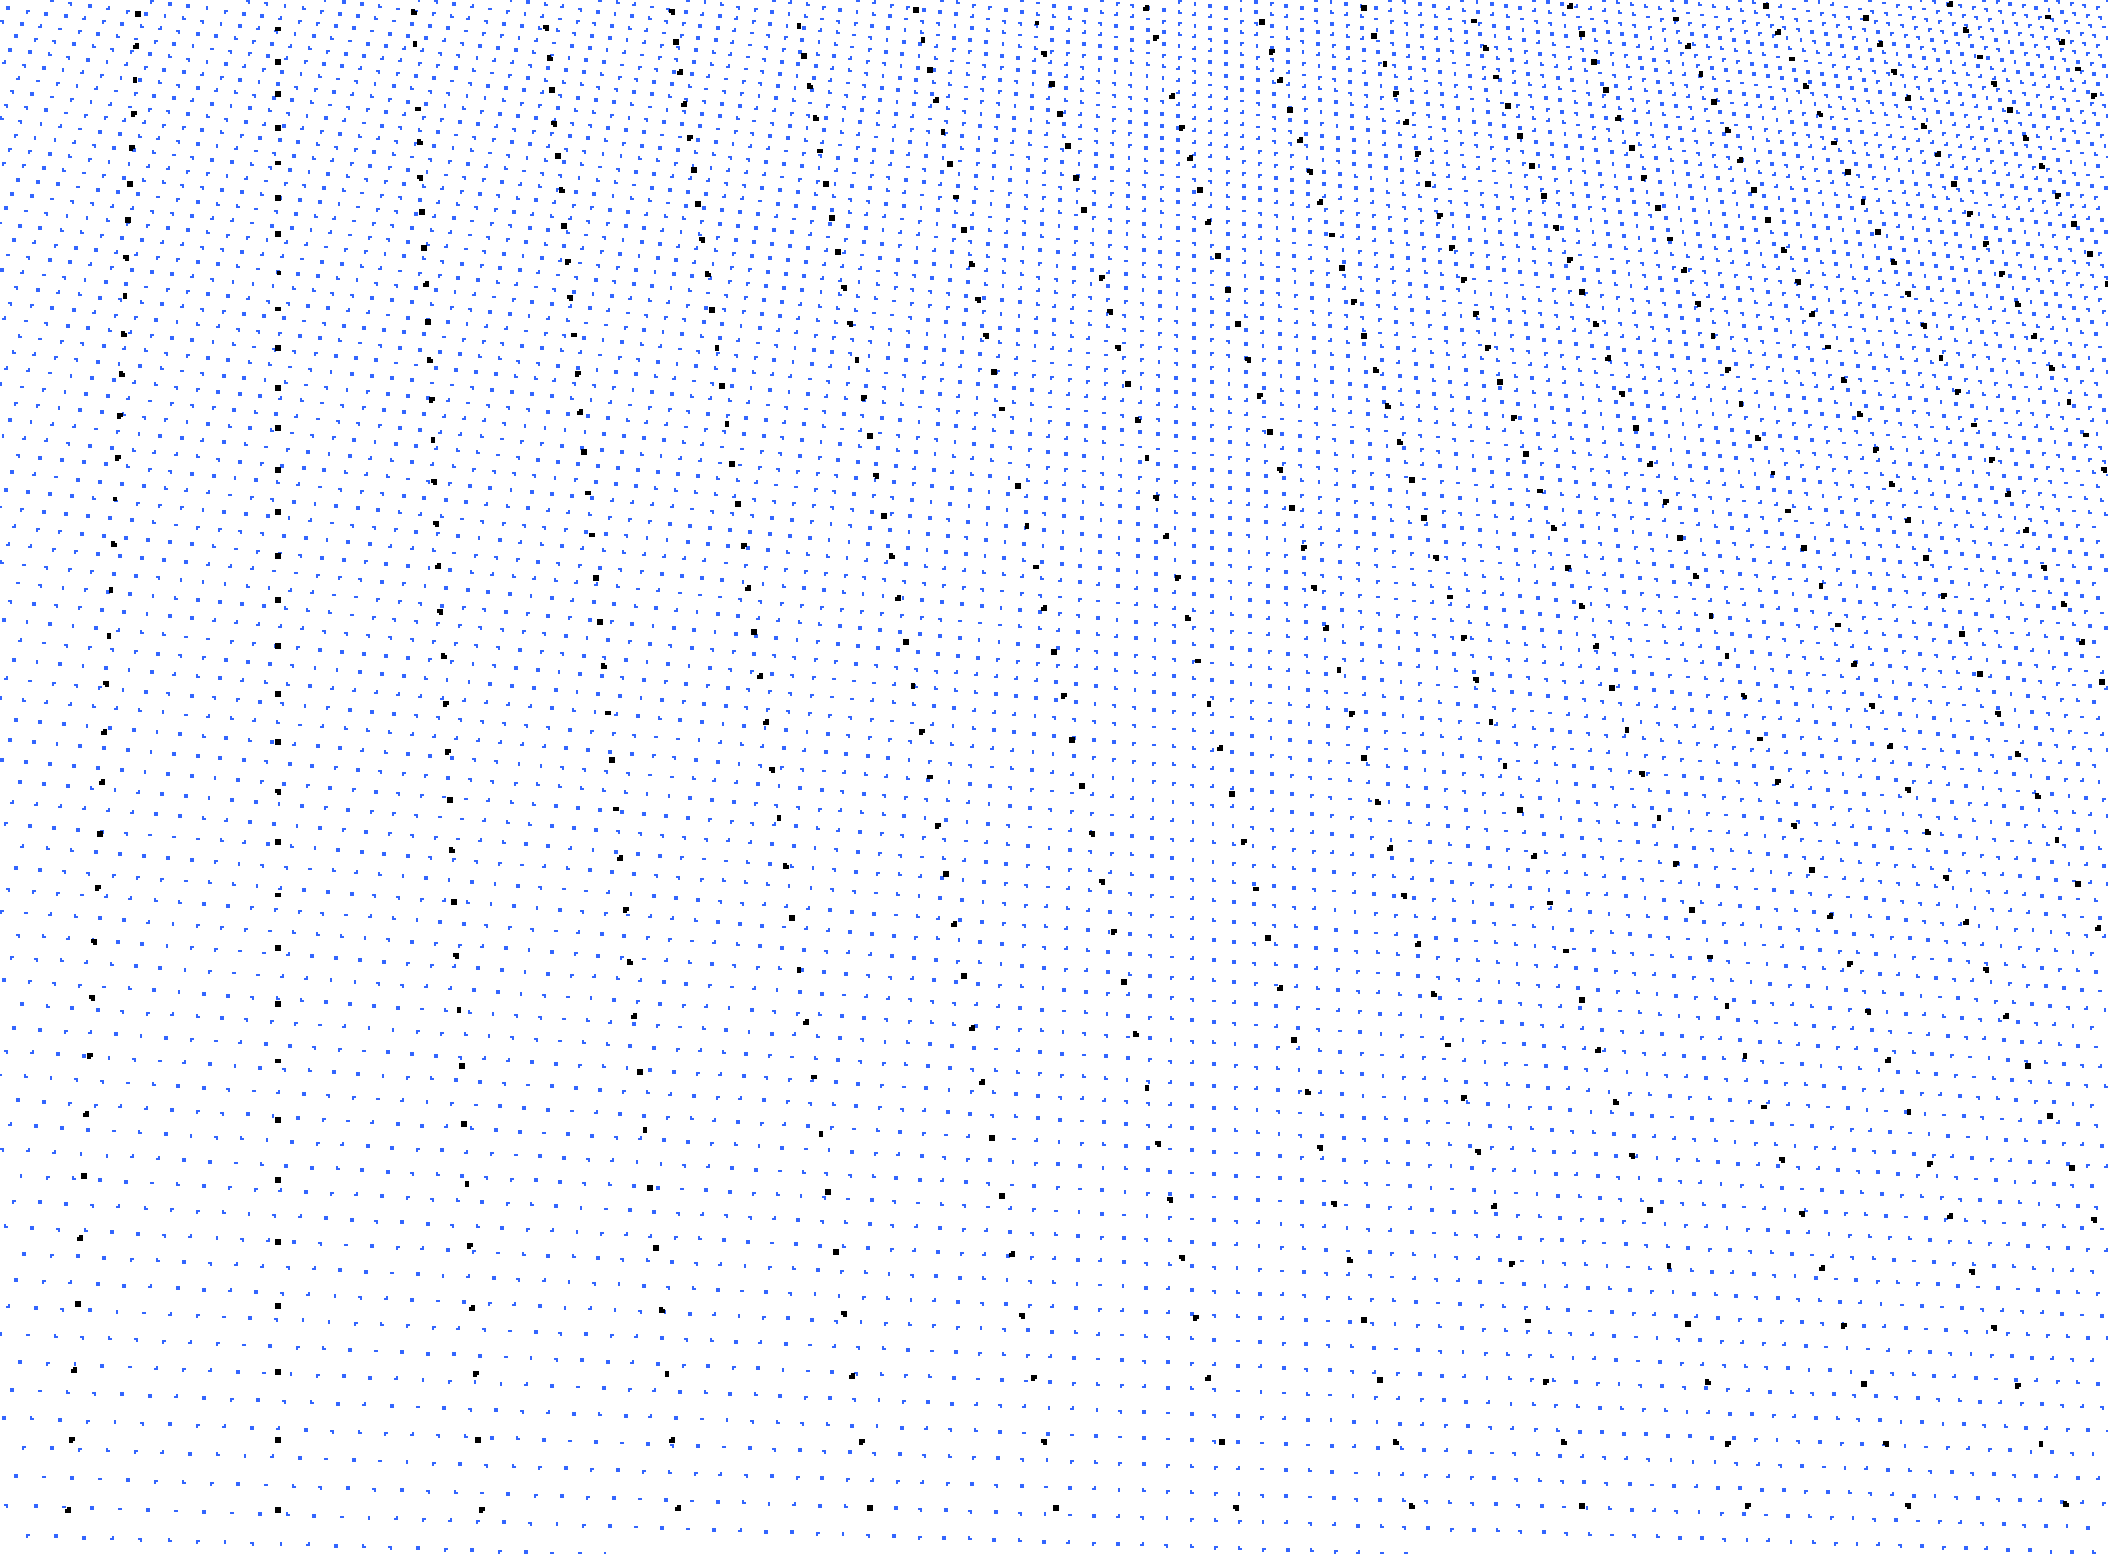
\includegraphics[width=.4\textwidth]{fig/closeup_pargrid.png}}%
}
\caption{Close-up view of parallelogram grid in $P$ (black), and sample point cloud $Q$ (blue)}
\label{fig:par_grid}
\end{figure}



\subsection{Adjusted own distance histogram}
As shown in the previous chapter, it is possible to calculate the range of the \gls{roi} of the histogram, using only the plane's normal vector $\vec{n}$ and the side length $p_l$ of the parallel projection camera. Here this result is used to to produce an \acrfull{aodh}, which still has the initial linear increase, for point clouds that are not planes.

When the surface is no longer a plane, $\vec{n}$ will no longer be constant, and can have a different value for each point. However for smooth surfaces on the model, the normal vector will remain approximatively constant on local regions of neighboring points, as can be seen on the close-up views in the previous sections. On these planar regions the parallelogram grid point dispersion reappears.

Under the assumption that most of the point cloud consists of such planar regions, its own distance histogram will be a superposition of the kinds of parallelogram grid histograms seen before, with an initial linear increasing segment.

\subsubsection{Multi-planes point cloud}
In order to test the shape of this superposition histogram, an artificially generated ``multi-planes'' point cloud is used. It consists of multiple planes places randomly in space at different orientations, projected using a parallel projection camera. An example with two planes is shown in figure \ref{fig:disks1}, shown with decreased point density.

The two planes are bounded to the shapes of disks. This does not have an effect of the histograms, and just makes the point cloud easier to visualize. If the bound was a square, it would change depending on the rotation of the plane on the axis pointing out of it.

Both planes have the parallelogram grid point dispersion. The example is chosen so that one plane is approximatively facing the camera while the other is more oblique, and has a lower $\rho$ and higher $l_\text{min}$ as a result. Figure \ref{fig:multiplane_cphist} shows the \gls{odh} for the two individual planes, and the superposition histogram for the entire multi-planes point cloud.

\begin{figure}[H]
\centering
\begin{subfigure}{.32\textwidth}
	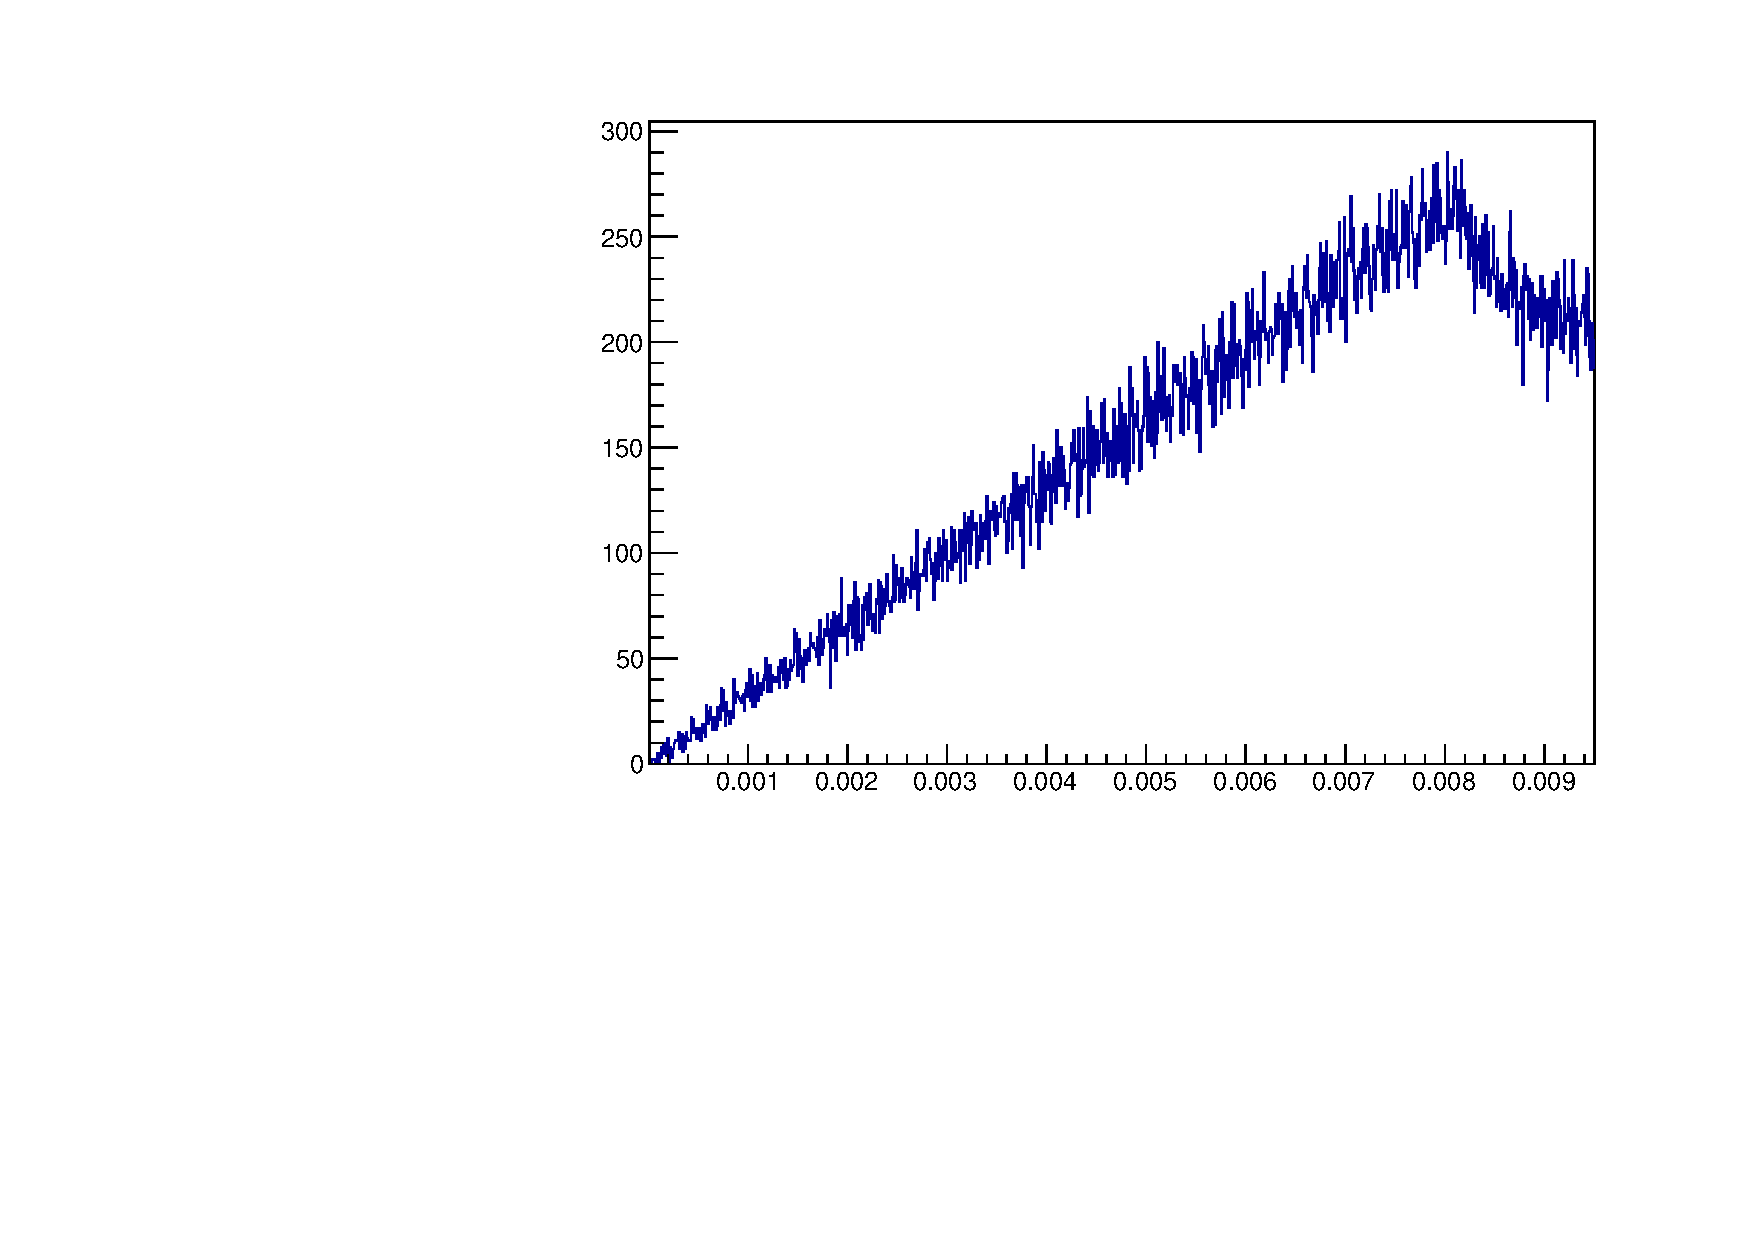
\includegraphics[width=\linewidth]{fig/orig_plane1.pdf}
	\caption{Oblique plane}
\end{subfigure}%
\begin{subfigure}{.32\textwidth}
	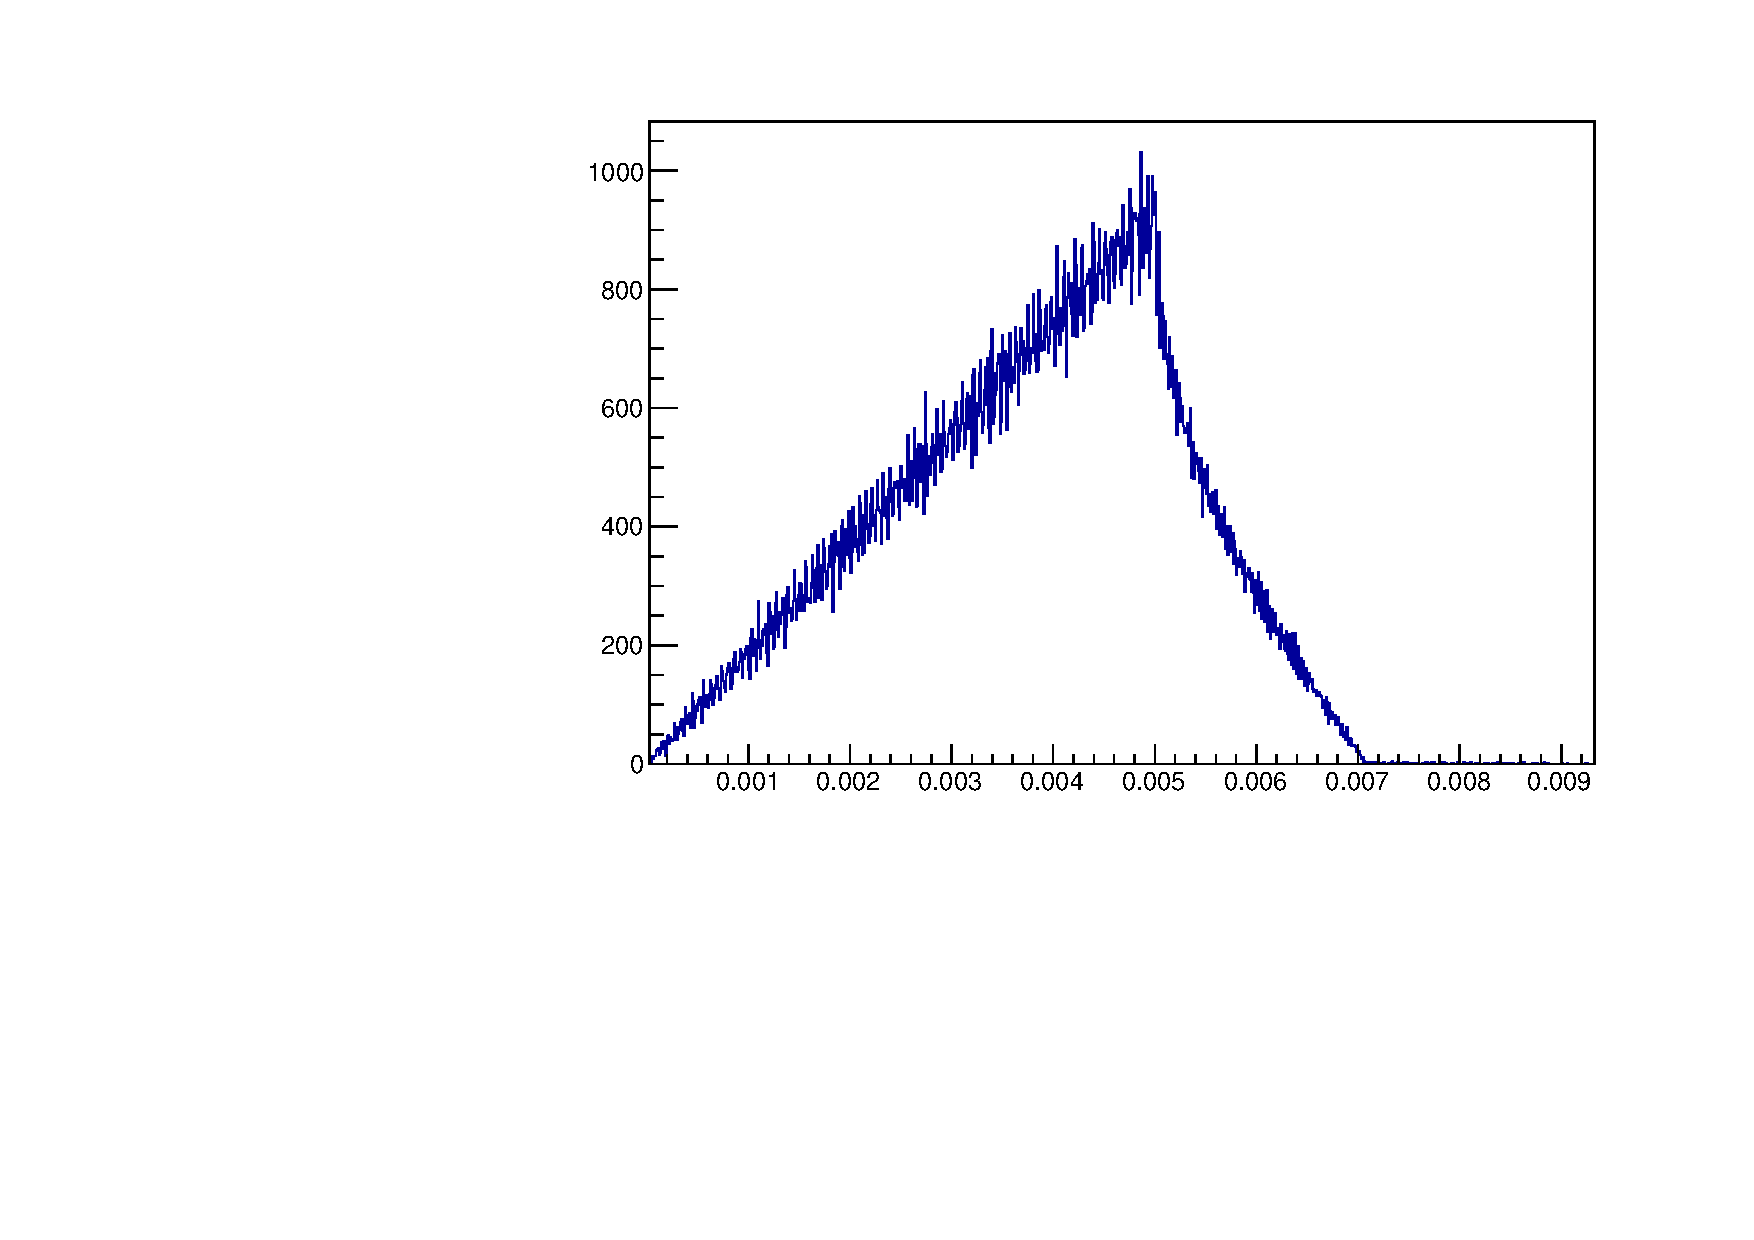
\includegraphics[width=\linewidth]{fig/orig_plane2.pdf}
	\caption{Parallel plane}
\end{subfigure}%
\begin{subfigure}{.32\textwidth}
	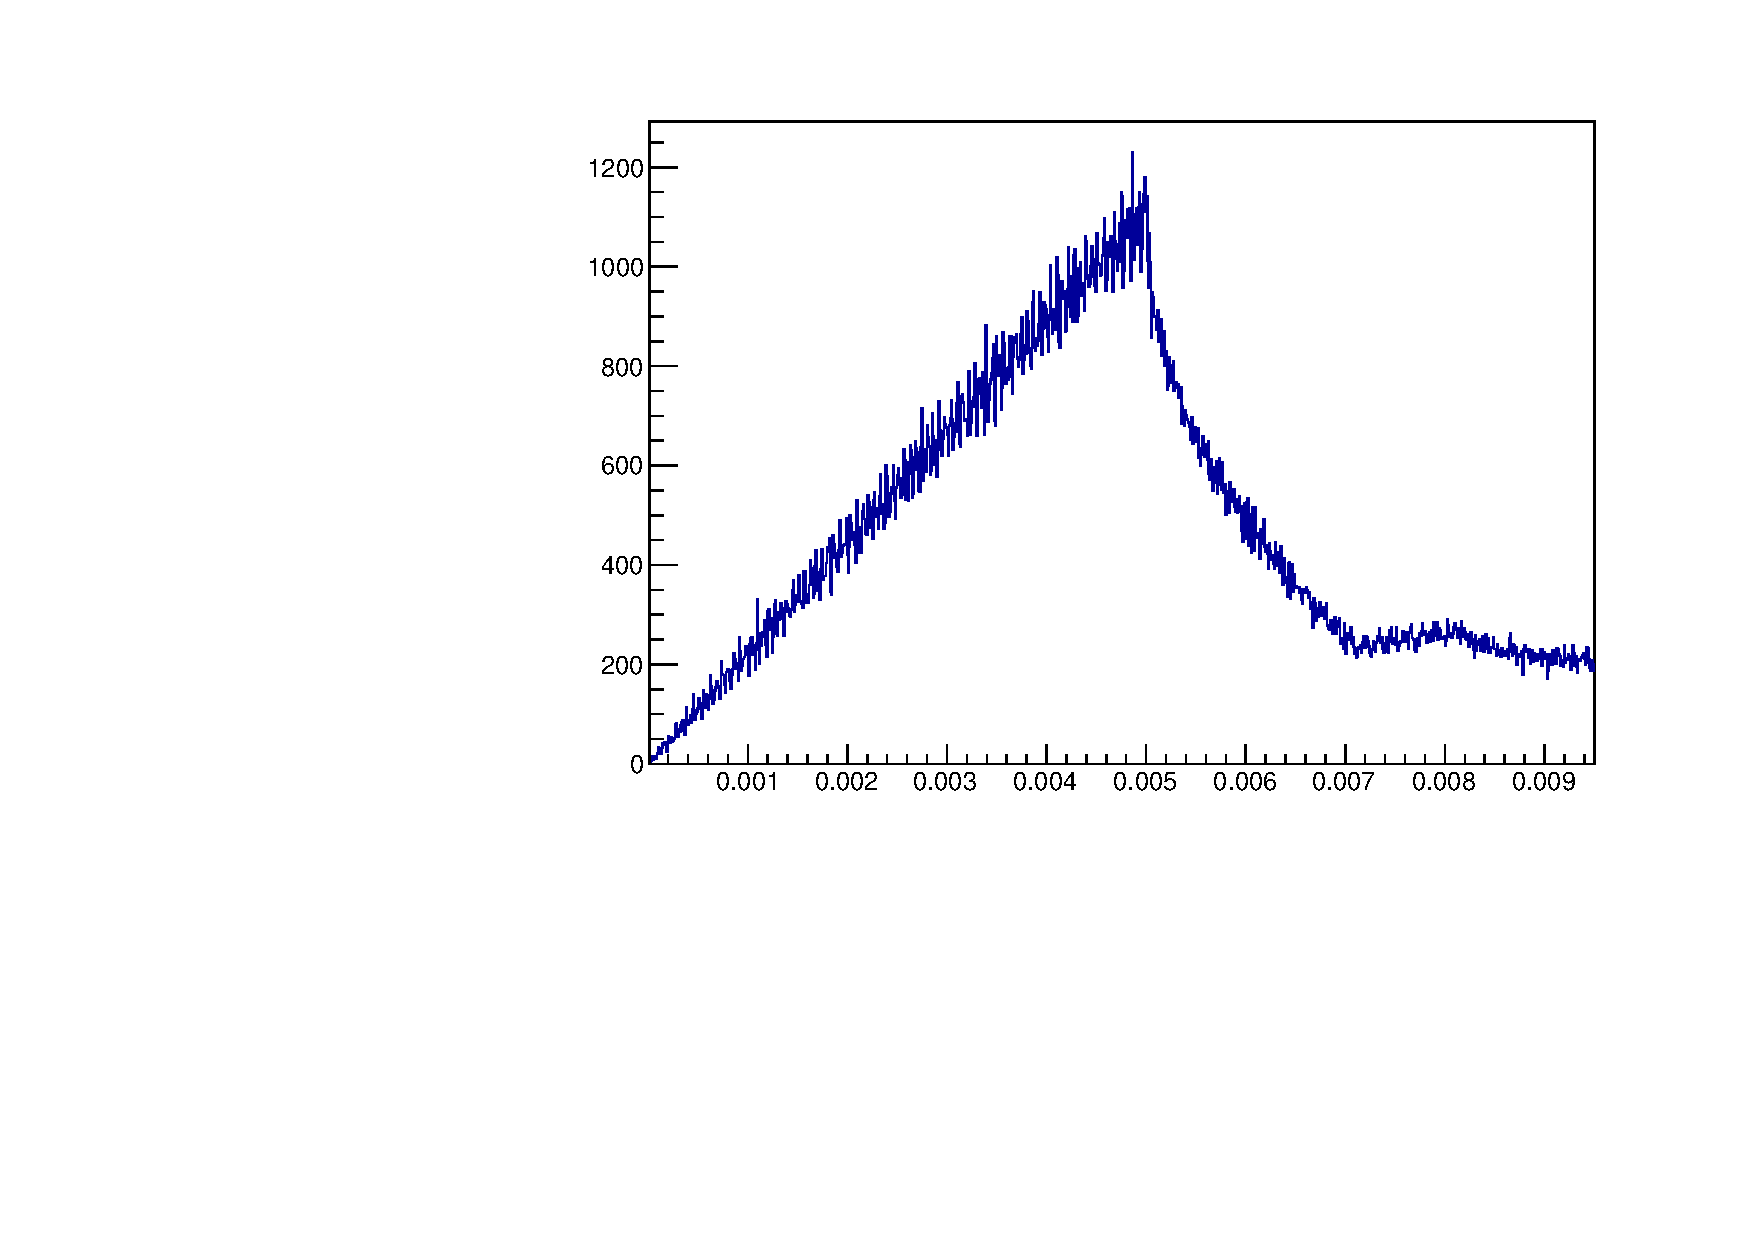
\includegraphics[width=\linewidth]{fig/orig_superposition.pdf}
	\caption{Superposition}
\end{subfigure}
\caption{\Gls{odh} for multi-plane point cloud $P$ (individual planes, and superposition)}
\label{fig:multiplane_cphist}
\end{figure}

It can be seen that the linear \gls{roi} of the superposition histogram ranges up to about $0.005$, which is the minimum of the ranges on the two individual histograms. The information from the remaining linear range of the oblique plane is lost.

\begin{figure}[h]
\centering
{
	\setlength{\fboxsep}{0pt}%
	\setlength{\fboxrule}{0.5pt}%
	\fbox{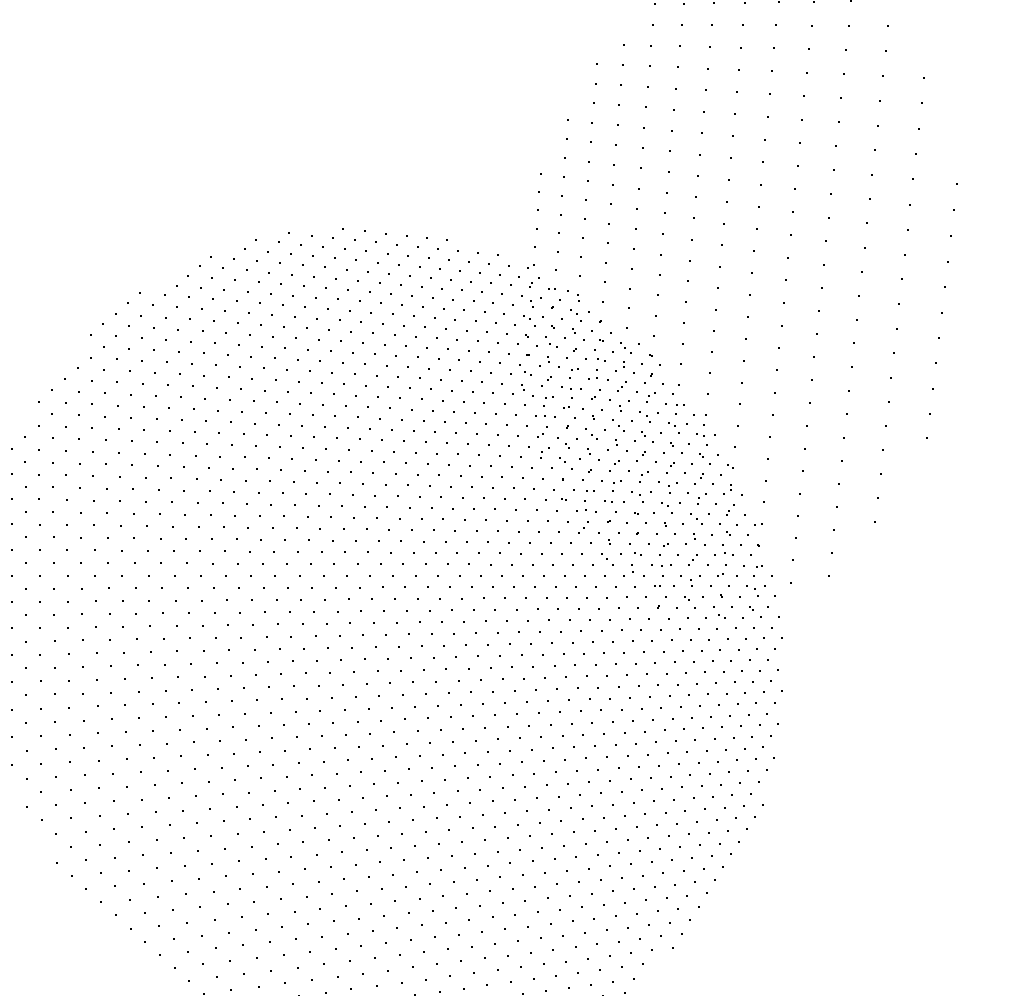
\includegraphics[width=.4\textwidth]{fig/disks1.png}}%
}
\caption{Example of multi-plane point cloud}
\label{fig:disks1}
\end{figure}


\subsubsection{Adjusted histogram}
The \gls{aodh} is created as follows: For each $q \in Q$, the closest point $p \in P$ is taken, for which $d = \|p - q\|$ is minimal. Then instead of $d$, the value $d' = \frac{2 \, d}{l_{\text{min}}(\vec{n})}$ is recorded in the histogram. $l_{\text{min}}$ is calculated from the normal vector $\vec{n}$ of $p$ using the approximation formula \ref{eq:pargrid_lmin} from the previous chapter. Samples are only added to the histogram when the threshold condition \ref{eq:pargrid_lmin_cond} is met.

All the histograms created from subsets of the point cloud that contain only regions of the surface with an approximatively constant normal vector $\vec{n}$, would have a linear increase until $d = \frac{1}{2} \, l_{\text{min}}(\vec{n})$. The adjusted own distance histogram is a superposition of all of these, distorted such that its \gls{roi} always ranges from $d' = 0$ to $d' = 1$.

The following figure \ref{fig:disks_adj} shows this \ghs{aodh}, in comparison to the non-adjusted \gls{odh}, for the same point cloud $P$. $P$ is a multi-planes as before, but with more planes. Figure \ref{fig:relief_adj} shows the same histograms where $P$ and $Q$ is a relief point cloud. It appears more irregular than the \gls{odh}, but the \gls{roi} contains a higher number of samples.
\begin{figure}[H]
\hspace*{\fill}%
\begin{subfigure}{.4\textwidth}
	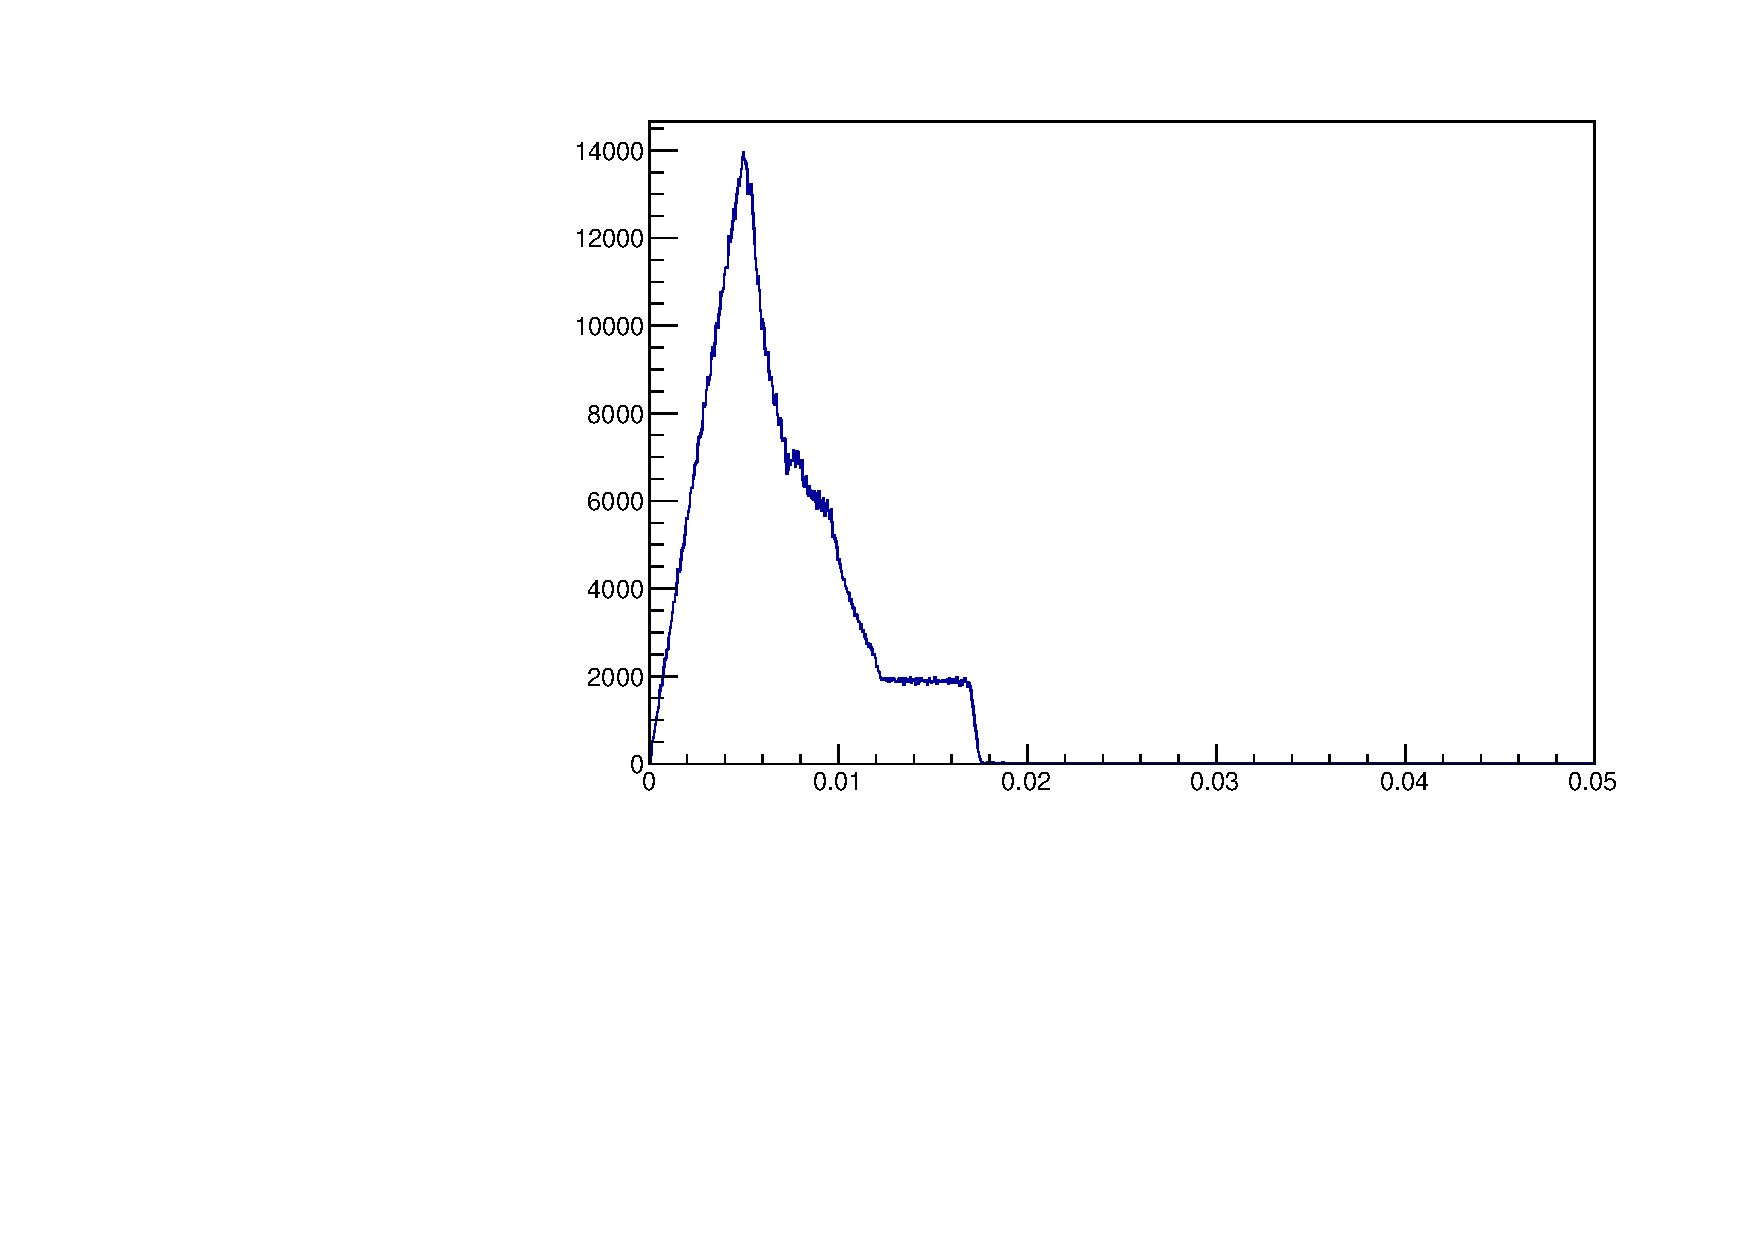
\includegraphics[width=\linewidth]{fig/disks_noadj.pdf}
	\caption{Non-adjusted histogram}
\end{subfigure}%
\hfill{}%
\begin{subfigure}{.4\textwidth}
	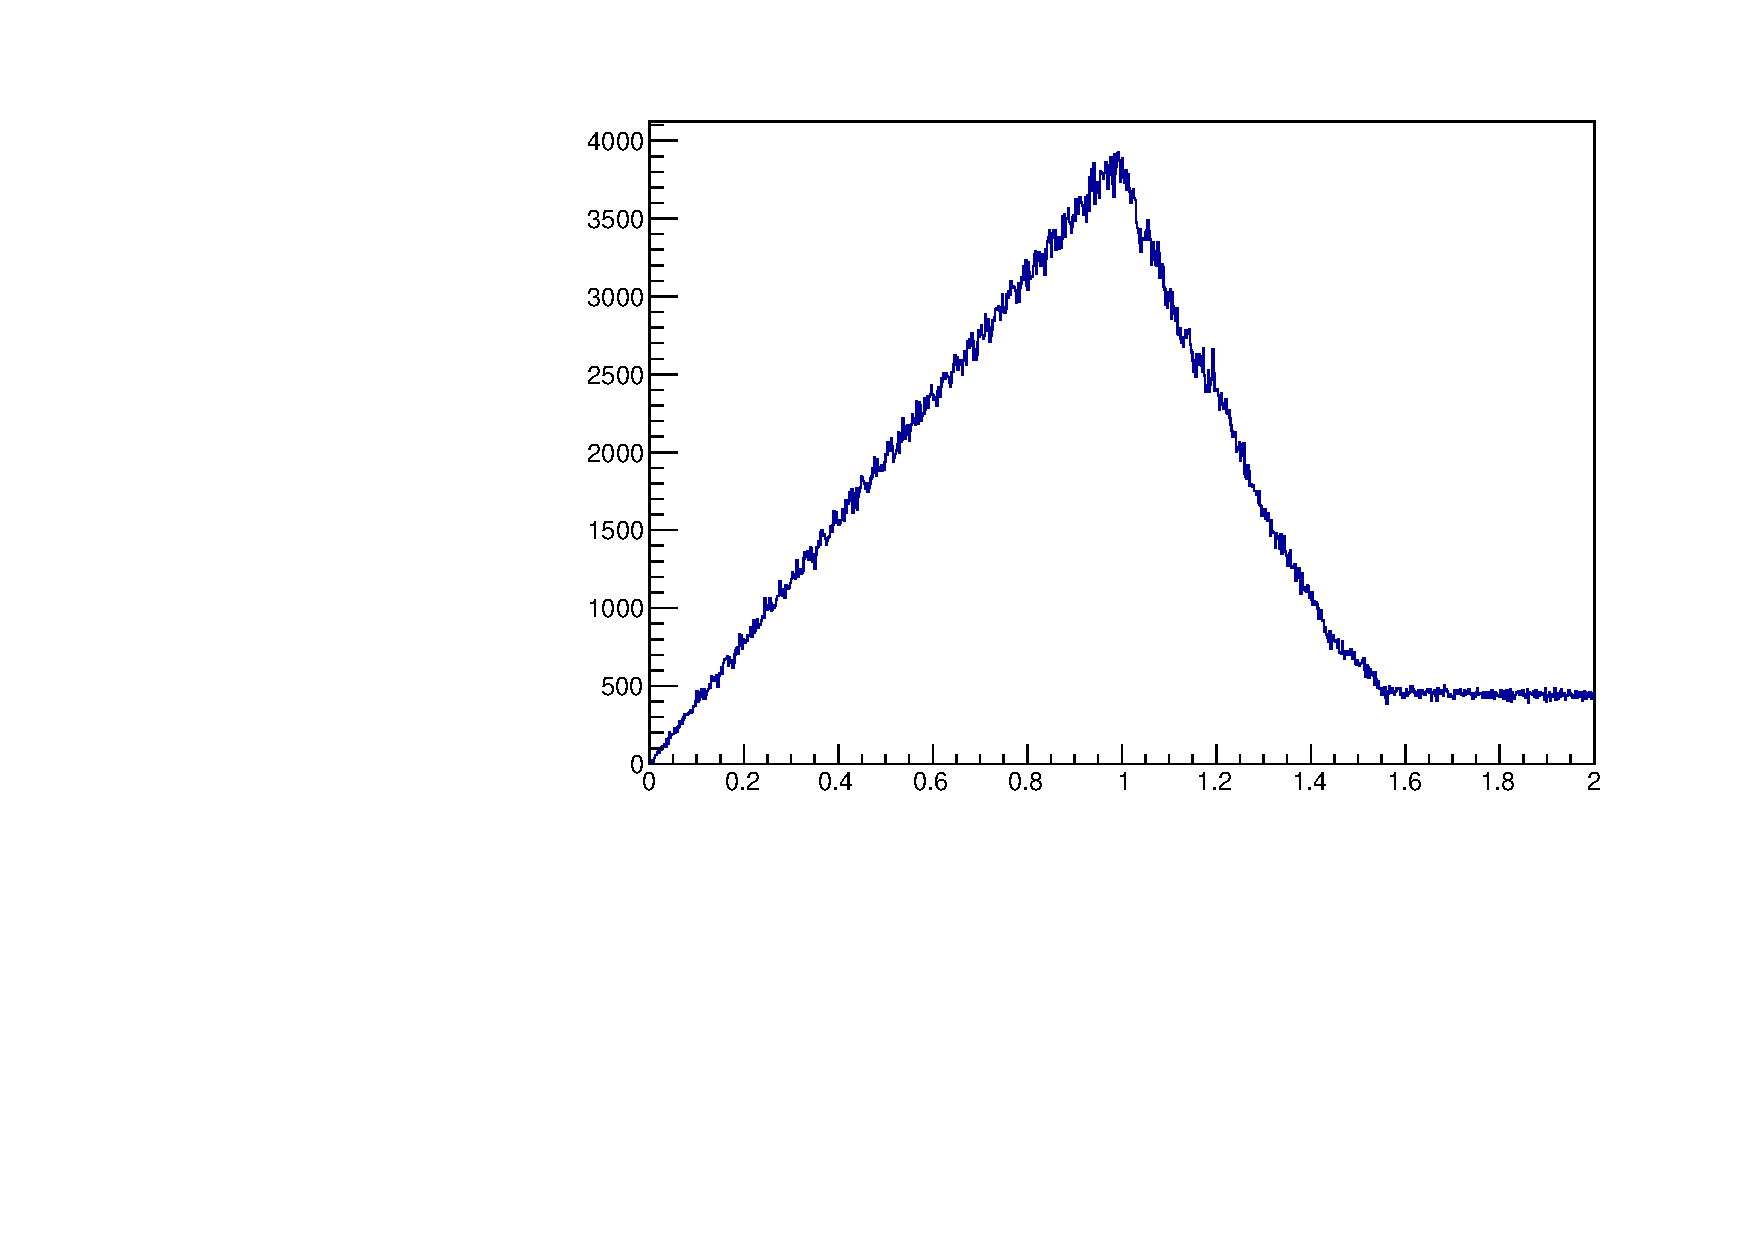
\includegraphics[width=\linewidth]{fig/disks_adj.pdf}
	\caption{Adjusted histogram}
\end{subfigure}
\hspace*{\fill}%
\caption{\Gls{odh}, and \gls{aodh} of $P$}
\label{fig:disks_adj}
\end{figure}

\begin{figure}[h]
\hspace*{\fill}%
\begin{subfigure}{.4\textwidth}
	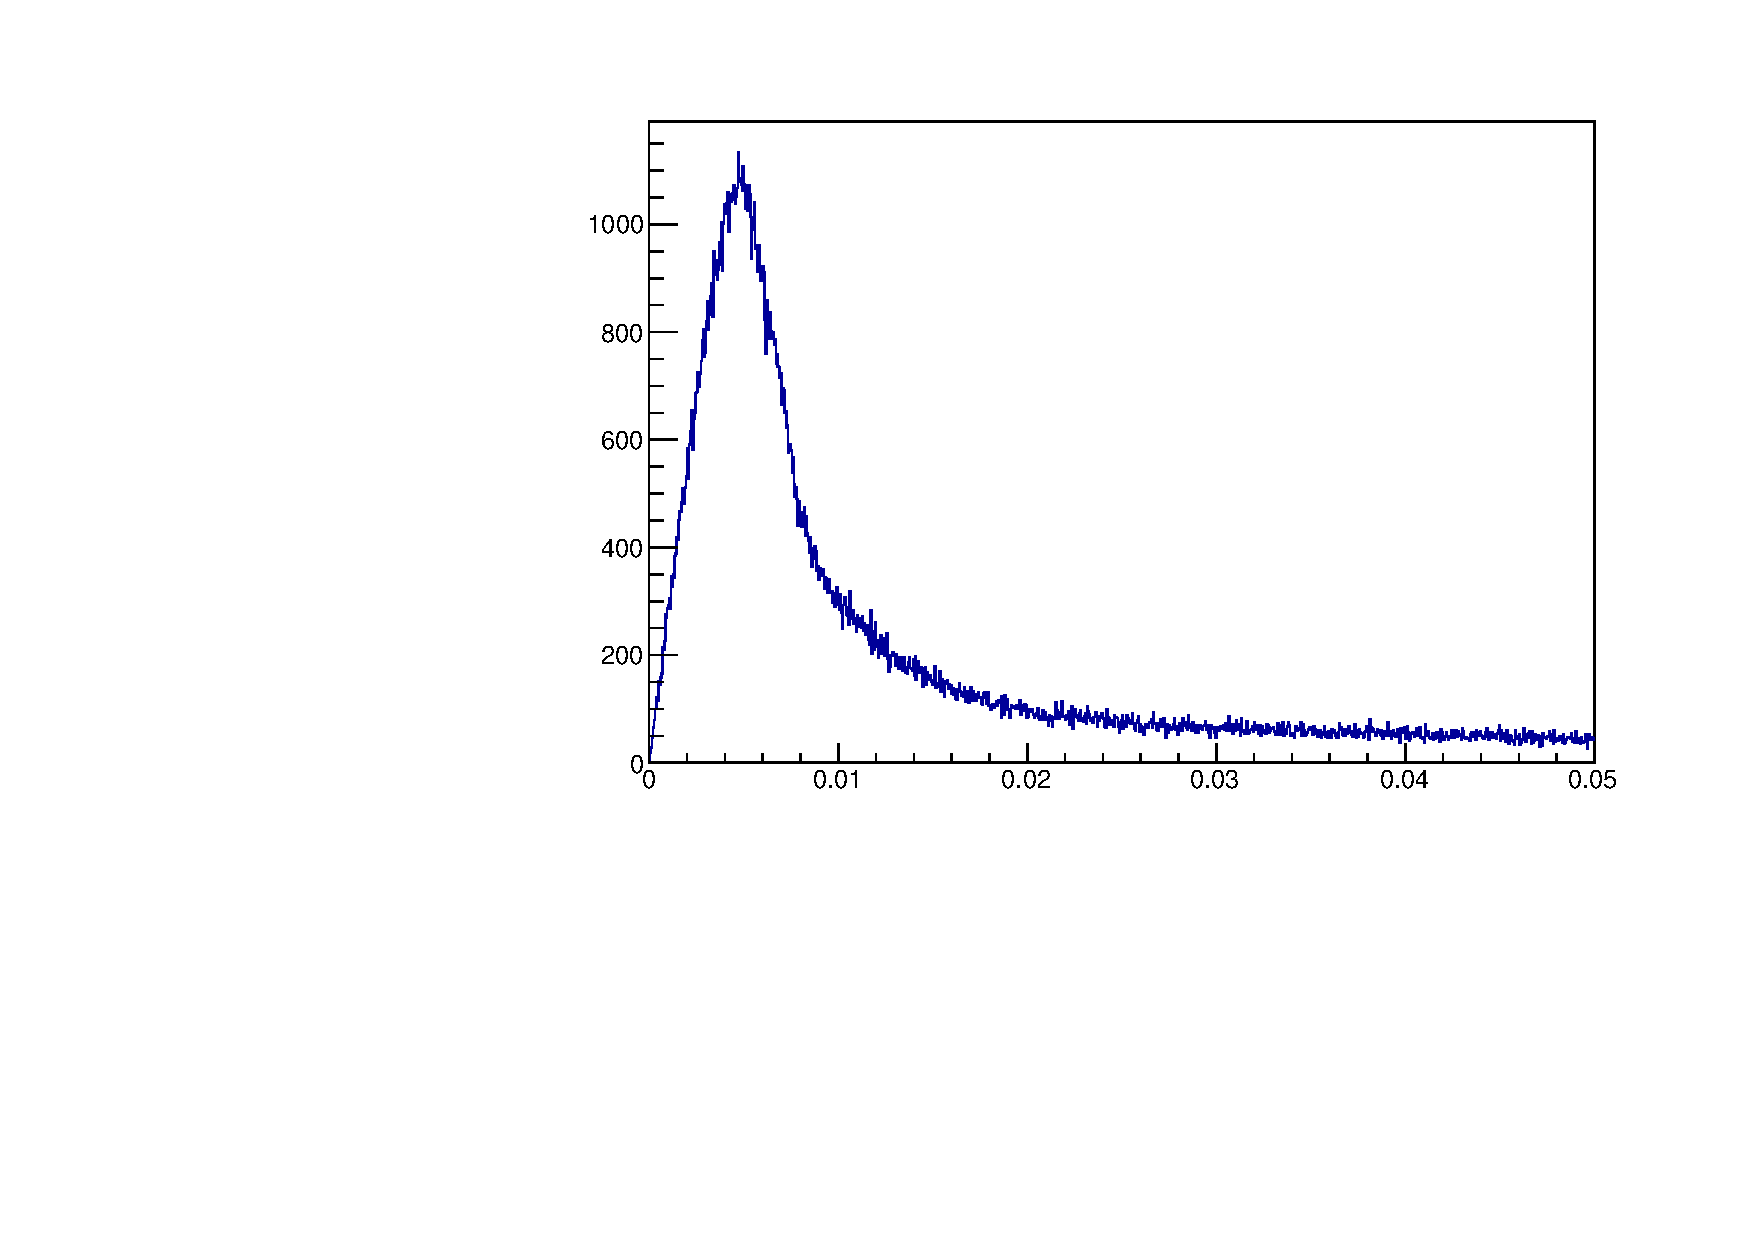
\includegraphics[width=\linewidth]{fig/relief_noadj.pdf}
	\caption{Non-adjusted histogram}
\end{subfigure}%
\hfill{}%
\begin{subfigure}{.4\textwidth}
	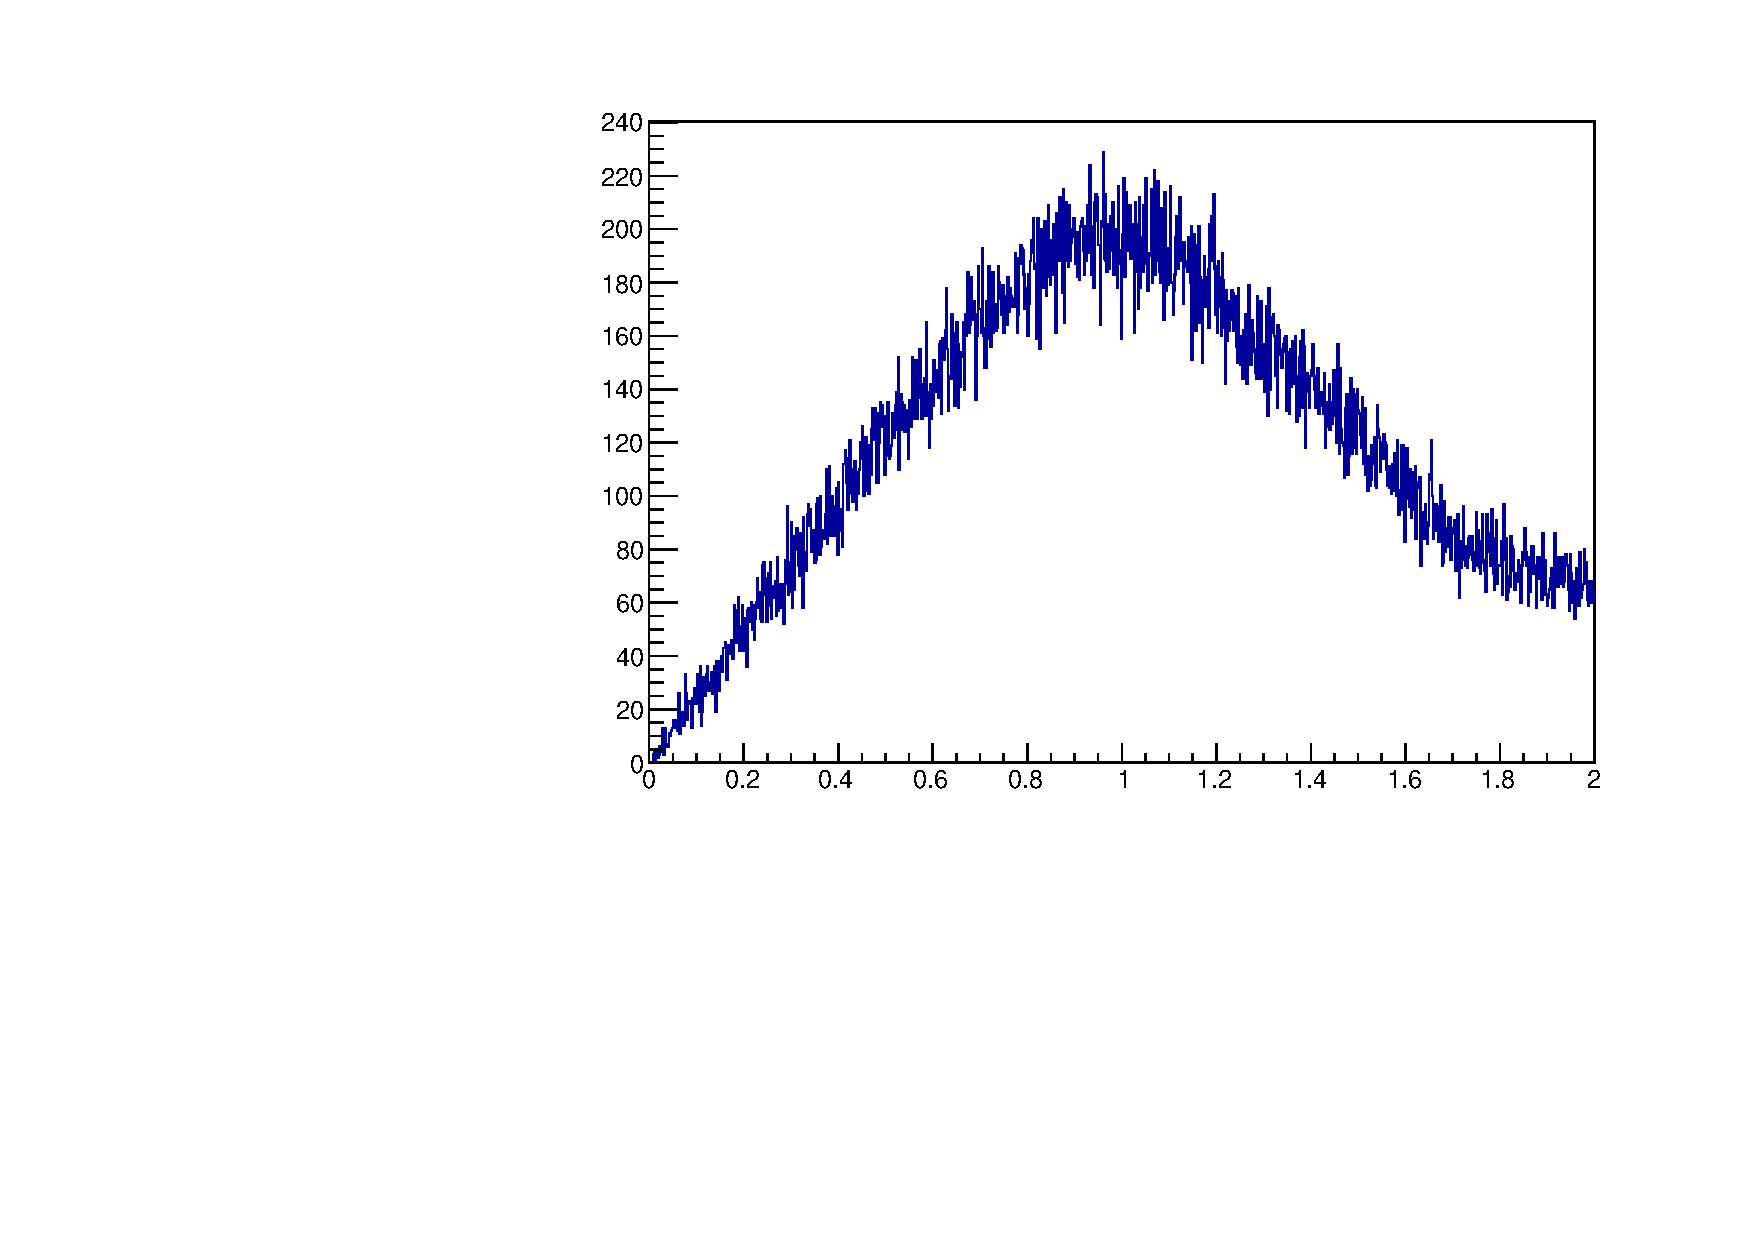
\includegraphics[width=\linewidth]{fig/relief_adj.pdf}
	\caption{Adjusted histogram}
\end{subfigure}
\hspace*{\fill}%
\caption{\Gls{odh}, and \gls{aodh} of relief point cloud}
\label{fig:relief_adj}
\end{figure}


\subsection{Occlusion and different bounds}
Point clouds obtained from real scans will not fully cover the surface due to occlusion, and any two point clouds $P$ and $Q$ will have different bounds. Thus there can be sample points $q$ on surface positions that are not covered by $P$, and vice versa.

It was assumed that the point dispersion on locally planar surface parts depends only on the local normal vector. Therefore when parts of the sample point cloud $Q$ are removed, it only decreases the quality of the histogram as there are less samples, but does not alter its shape.

However when parts of the model point cloud $P$ are removed, for sample points $q \in Q$ that fall within these regions, the closest point $p \in P$ will be much farther away. As a result much greater distances are recorded, than for the samples falling within the parallelogram grid of $P$.

These distance values add more samples on the right side of the histogram, and do not affect the shape of the \gls{roi} of the histogram.

In the histograms on figure \ref{fig:relief_adj}, $P$ is a sideways view-point of the relief model, and it can be seen that the \gls{odh} contains samples at greater distances, at a low but near constant rate. When zoomed out, this extends to a much longer range.


\subsection{Sample for real point cloud}
When $P$ is not an artificially generated point cloud but is taken from a 3D scan, the sample $Q$ cannot easily be constructed as the surfaces are unknown.

Using the scan as sample and a randomly down-sampled version of it as model is not possible, because the properties of the point dispersion get removed. When the range image is down-sampled in image space the point dispersion pattern is preserved, but now sample points will always either coincide with model points, or fall into the same relative positions in the parallelograms.

The histogram of the nearest neighbor distances, that is, the distance from each point in $P$ to the closest point in $P$ except for itself, does not produce an \gls{odh}.

One approach to construct a higher resolution sample $Q$ from the point scan $P$ is the following:
\begin{enumerate}
\item $P$ is supposed to be a range image. Its camera position is at the origin of its coordinate system. As shown in section \ref{sec:estimate_proj_par}, $p_l$ and $l_{\text{min}}$ can be estimated from the point cloud.
\item All points from $P$ which no not satisfy the threshold condition for obliqueness \ref{eq:pargrid_lmin_cond}, and the points for which the local surface curvature is too large, are removed.
\item $Q$ is initialized to an empty point cloud.
\item For the \gls{aodh}, points with $d > \frac{1}{2} l_{\text{min}}$ will fall outside its \gls{roi}, so $Q$ does not need to include those.

A copy $P'$ of $P$ is constructed, and each of its points $p$ is randomly displaced along its tangent plane. The tangent plane is calculated using the point's normal vector. The random displacement along the polar coordinates $r$ and $\theta$ on this plane, centered on the point $p$, is done according to an uniform distribution with  $r \in [0, \frac{k}{2} l_{\text{min}} ]$ and $\theta \in [0, 2 \pi]$, where $k \geq 1$ (and not smaller than $1$). It can be set to a greater value to compensate for when the scanner rays are actually not parallel.
\item $P'$ is fused into $Q$. Then step $4$ is repeated, for a total of $N$ times.
\end{enumerate}
The resulting sample point cloud $Q$ now has $N$ times the number of points than $P$, its still lie on the object surfaces (assuming $P$ is locally planar in the direct neighborhood of its points), and they are uniformly distributed around the points.

\subsubsection{Results}
The \gls{aodh} obtained from the dessus-de-porte point cloud as $P$, and a sample point cloud $Q$ constructed from it with this method, is shown in \ref{fig:ddp_adj}. It still shows the linear increase in the \gls{roi}. However this result is not surprising, since $Q$ was specifically constructed to have an uniform distribution of the displacement radii $r$ on the tangent planes.

The idea is that if another, higher resolution scan of the same object is used as $Q$, the linear increase should also be present, but only when the point clouds are perfectly aligned. Measuring how linear the \gls{roi} is should give an indication of how well $P$ and $Q$ are aligned.

\begin{figure}[h]
\centering
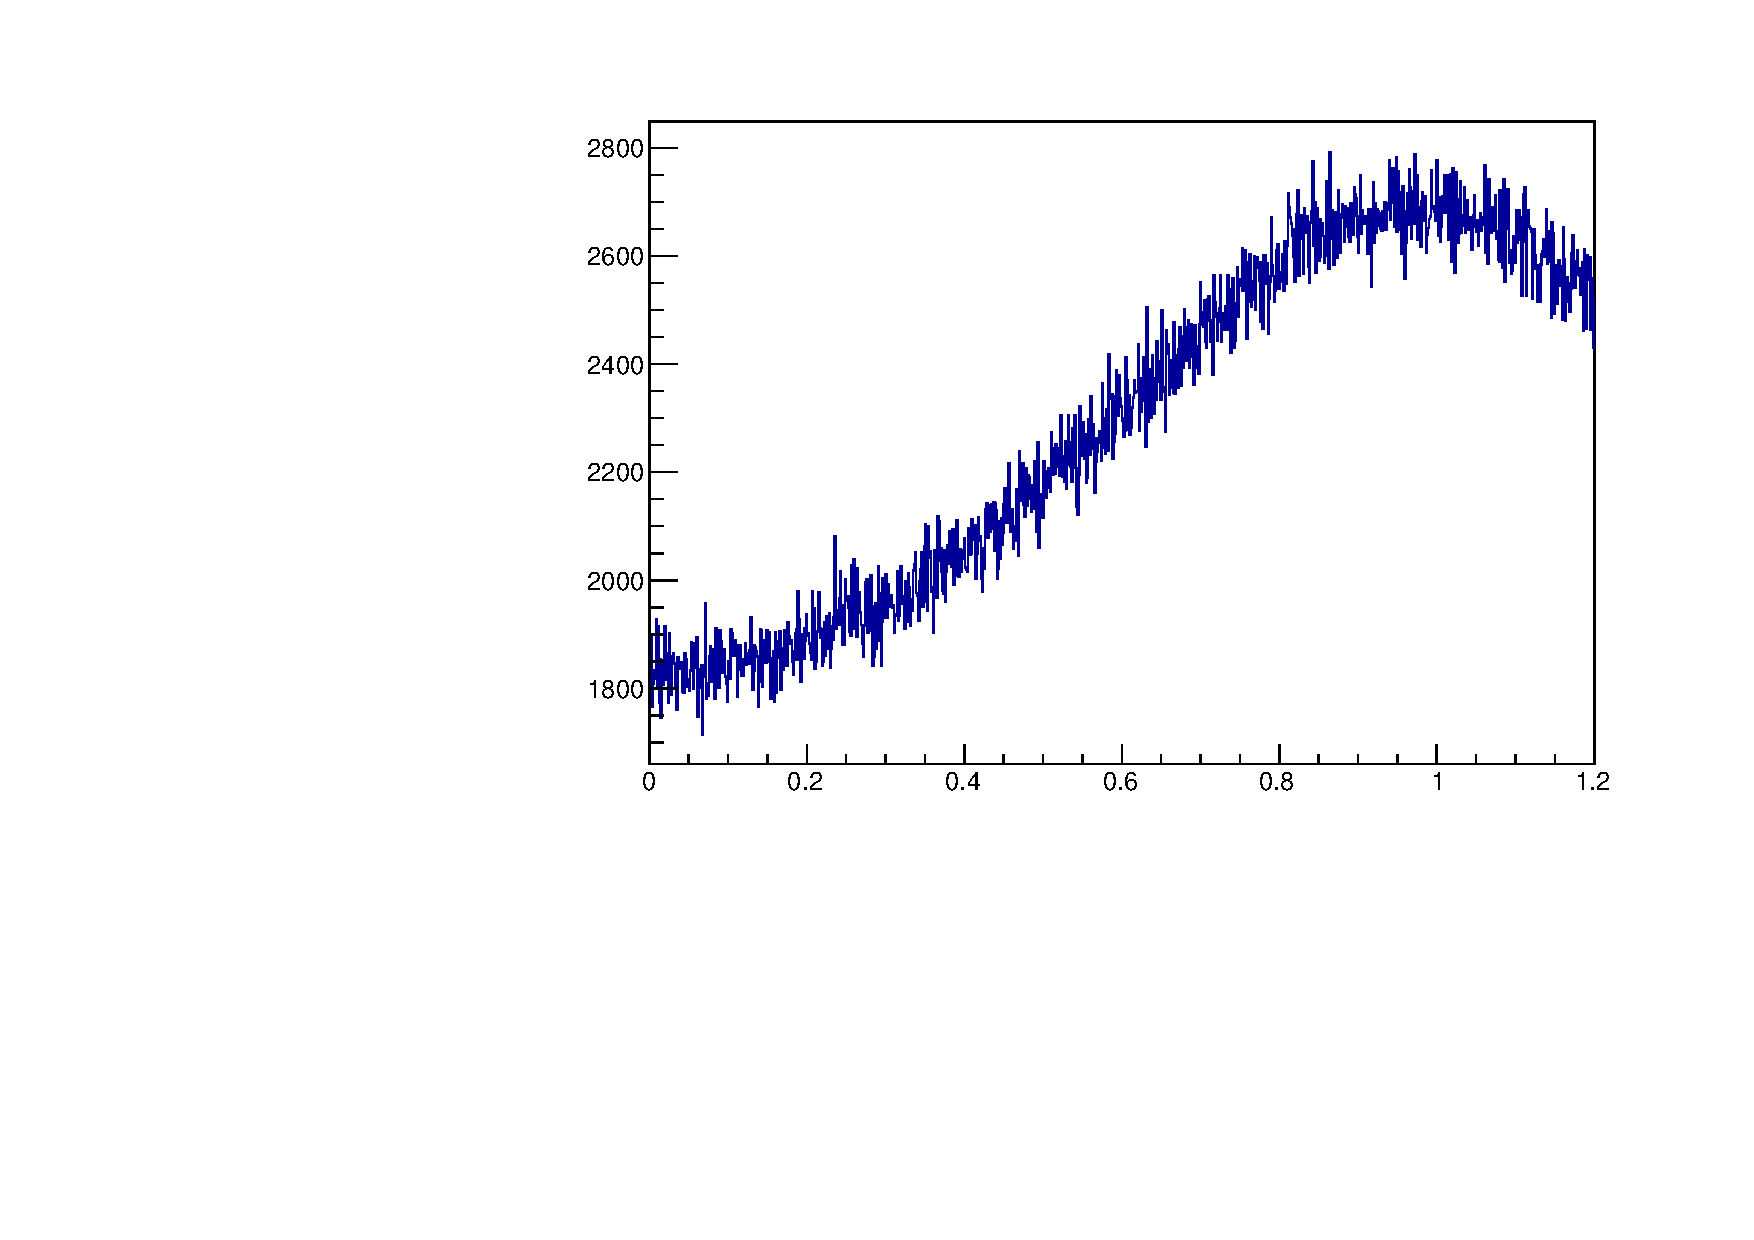
\includegraphics[width=.4\textwidth]{fig/ddp_adj.pdf}
\caption{\Gls{aodh} for dessus-de-porte $P$ from constructed sample point cloud $P$}
\label{fig:ddp_adj}
\end{figure}

\FloatBarrier

\section{Cross distance histogram}
Up until now $P$ and $Q$ were considered to represent the same surface and be perfectly aligned. For the \gls{cdh} this last constraint is removed, so there is a rigid transformation $\matr{M}$ which aligns $P$ to $Q$.


\subsection{Adjusted histogram}
As before the \gls{acdh} is constructed from the distances of the sample points $q \in Q$ to their closest point $p \in P$.

To reduce the number of wrong correspondences, they are only accepted when the normal vectors of $p$ and of $q$ are \emph{compatible}, that is, the angle $\arccos \vec{n}(p) \, \vec{n}(q)$ is below a fixed threshold value. If the normals point in different directions, the points do not represent the same locations on the surface. Also, correspondences where $d(p, q)$ is above a fixed maximal distance are rejected.

Because the surfaces are no longer perfectly aligned, the distribution of the distances $d = d(p, q)$ will be different. Whenever $q$ is at a distance from the surface of $P$ on which $p$ lies, $q$ no longer falls into the two-dimensional parallelogram grid, and $d$ will be larger. Hence the more $\matr{M}$ deviates from $\matr{I}$, the more the distribution of $d$ will deviate from the one from the \gls{aodh}, and it will no longer have the characteristic linear increase from $d = 0$ to $1$.


\subsection{Rejection histogram}
In addition to this \gls{acdh} the \acrfull{arcdh} will be considered. Here the sample points $q \in Q$ are projected onto the surface of $P$, and then the distance from this \emph{projected point} $q_{{proj}}$ to $p$ is measured and recorded into the histogram. The projected point is calculated using the normal vector of $p$, denoted $\vec{n}_p$:
\begin{equation}
\vec{q}_{\text{proj}} = \vec{q} - \left[ \vec{n}_p (\vec{q} - \vec{p}) \right] \vec{n}_p
\end{equation}
And the distance $d_{\text{proj}} = \| \vec{q}_{{proj}} - \vec{p} \|$ is recorded. The vector $\vec{q}_{{proj}} - \vec{p}$ is also called the \emph{rejection}.

$p$ is still computed as the closest point to $q$ and not to $q_{\text{proj}}$, as otherwise the closest point algorithm would have to be run twice. This should not have a noticeable impact on the results.

Assuming that $\vec{n}_p$ is accurate, $\vec{q}_{\text{proj}}$ is placed on the surface, and as a result the histogram should take on the shape of the \gls{aodh}. However the sample points $vec{q}_{\text{proj}}$ are no longer as evenly distributed. When $Q$ is rotated relative to $P$, they will tend to cluster together more in areas further from the center of rotation. As shown before in \ref{sec:disp_sample_pts}, more variance in the density of the sample points leads to a more jagged histogram.

Also, unlike the \gls{acdh}, this \gls{arcdh} is, ideally, based solely on the dispersion patterns of the points of the surface, and does not take the distances of the surfaces of $P$ and $Q$ into account.


\subsection{Measure of alignment}
In order to find out how the \gls{acdh} and \gls{arcdh} change when a small rigid transformation is applied to $P$, several small translations and rotations were tested. The model is same artificial relief model as in the end of the previous section. For $P$ it is projected from a sideways angle. Results are shown and commented in appendix \ref{sec:relief_small_trans_exp}.

The goal was to construct a numerical error metric which indicates how well $\matr{M}$ aligns $P$ and $Q$. For this the adjusted cross distance histogram is compared to the hypothetical linear increase from $d = 0$ to $1$, using one of the measures described in section \ref{sec:histogram_comp}.

Figure \ref{fig:hist_tri} shows a observed histogram, along with the expected linear increase. The samples with $d > 1$ are discarded. The bins of the histogram are set to have equal width $w$. On the figure $w$ is exaggerated, and neither the observed values nor the expected values (i.e. the blue line) are drawn with the real bin size.

\begin{figure}[h]
\centering
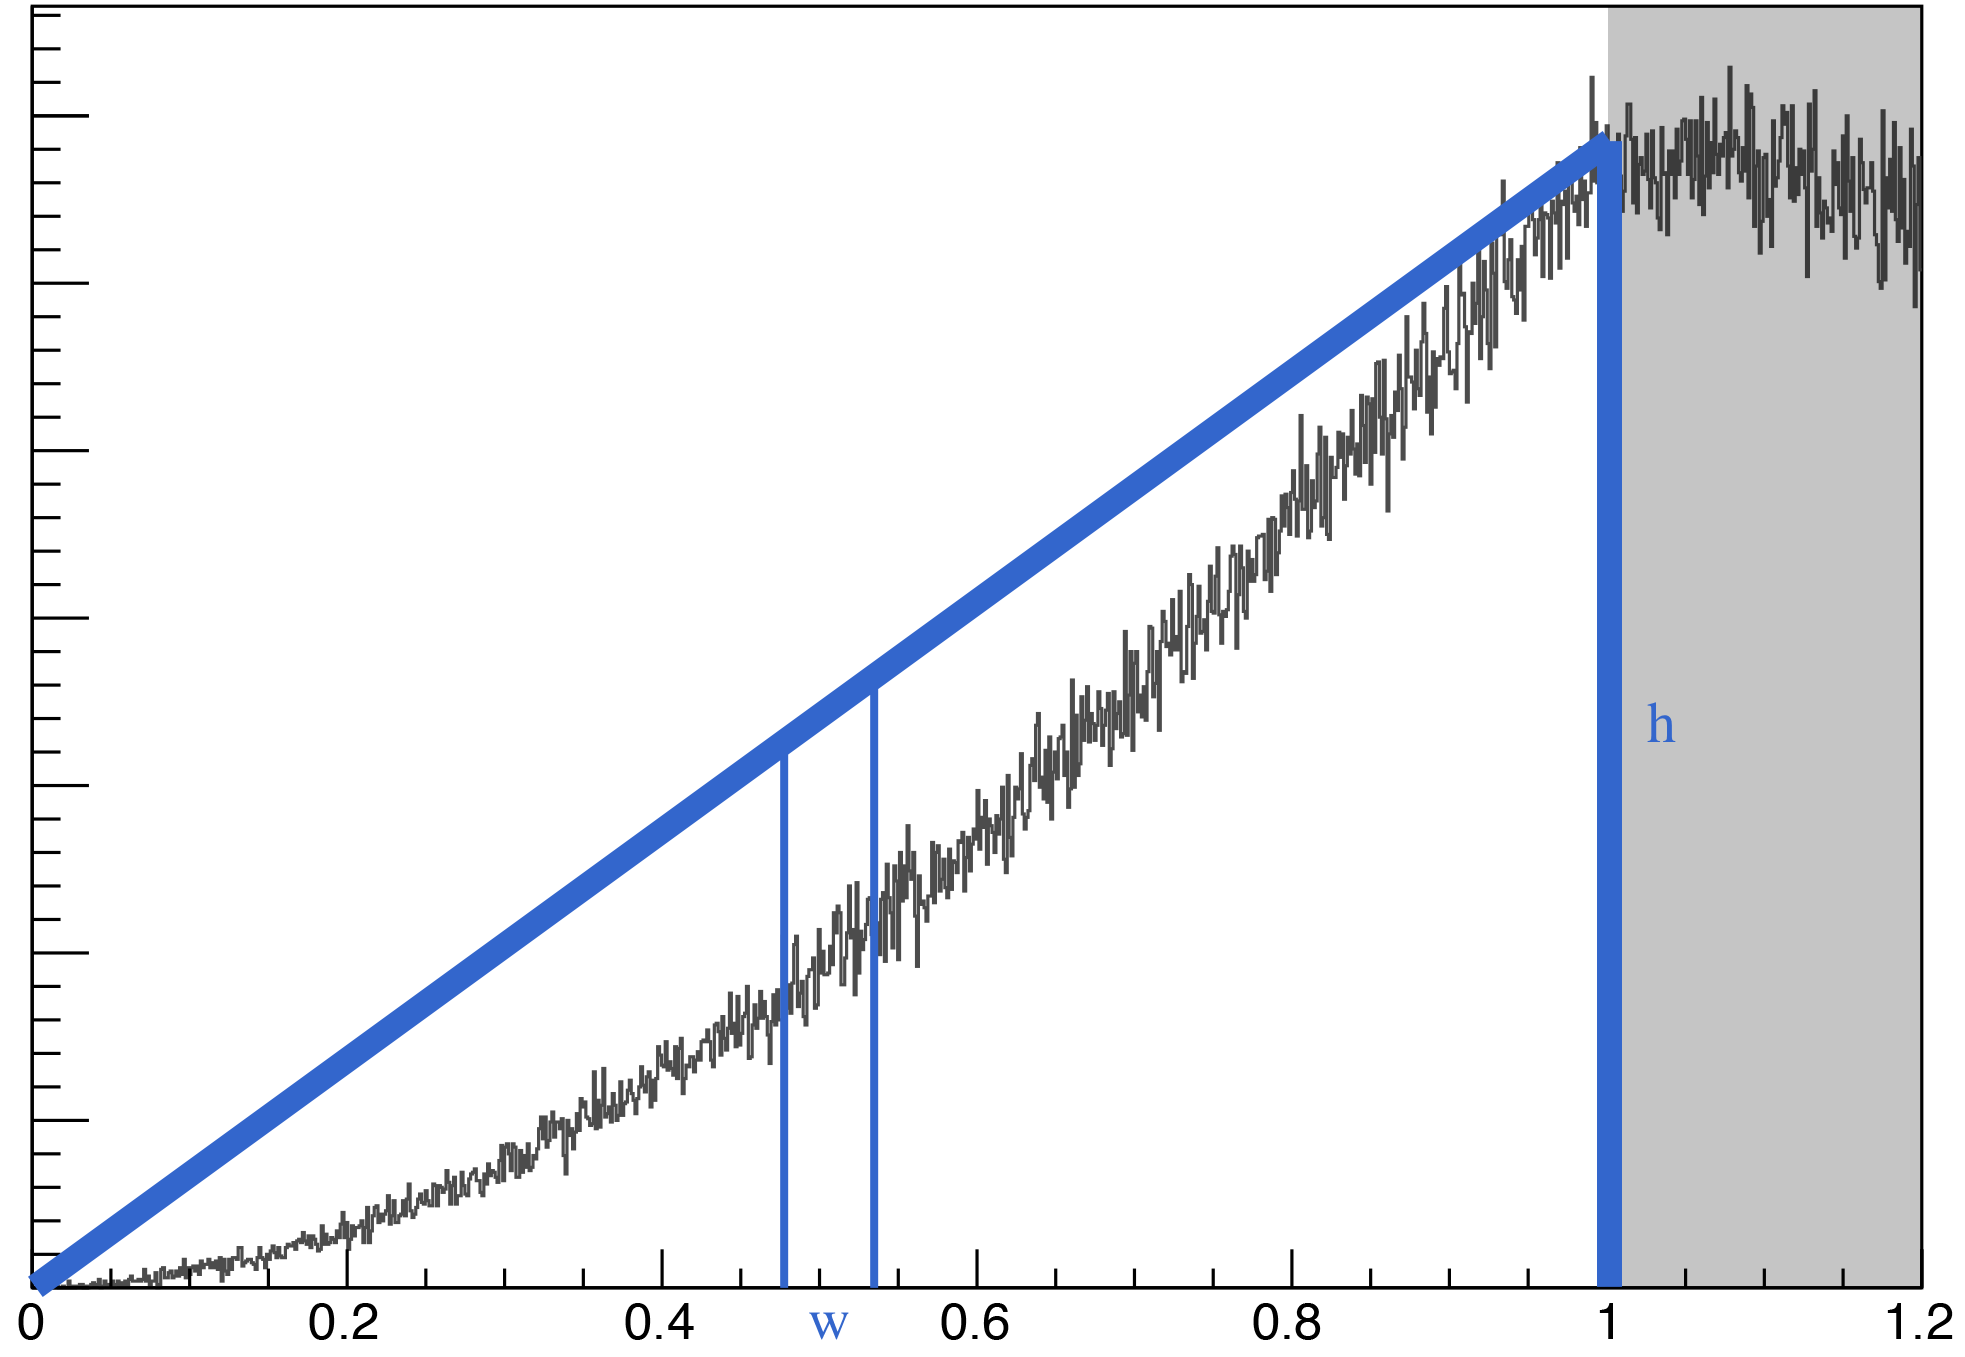
\includegraphics[width=.5\textwidth]{fig/hist_tri.png}
\caption{Representation of observed and expected histogram}
\label{fig:hist_tri}
\end{figure}

The ``height'' $h$ of the histogram at $d = 1$ is unknown, and depends on the bin width. Because the range is $1$, the area under the histogram curve is equal to the total number of included samples $n$. If the shape is precisely the linear increase, it should be equal to the area of the triangle formed by the blue lines, which is $A = \frac{1}{2} \times 1 \times h = \frac{h}{2}$. So $h = 2 \times n$.

The number $o_i$ of observed values which fall into one bin of width $w$, centered at $d_i$, is the number of samples $d$ such that $d_i - \frac{w}{2} < d < d_i + \frac{w}{2}$. The corresponding expected value is then calculated as the area of the rectangle of with $w$ and height $\frac{d_i}{1} \times h$, so $e_i = w \times d_i \times 2 \times n$.

Both values are normalized by dividing them by $n$. The expected and observed values used to compare histograms are
\begin{equation}
o_i = \frac{1}{n} \times N\left(d_i : \frac{w}{2} < d < d_i + \frac{w}{2}\right)
\hspace{7mm} \text{and} \hspace{7mm}
e_i = 2 \, w \, d_i
\end{equation}

Using this, the \emph{chi-squared} error metric is calculated. Let $e_{\chi}$ be this chi-squared measure when applied on the \gls{acdh}, and $e_{r,\chi}$ its equivalent on the \gls{arcdh}.

When the observed histogram increases linearly in the \gls{roi}, $e_{\chi}$ and $e_{r,\chi}$ should be zero. Otherwise, it should be larger. So this new error metric should have its minimal value when $\matr{M}$ perfectly aligns the point clouds.

These error metrics, were compared with the mean absolute error taken with the closest point criterion. The same relief point cloud is used for both, and the error metrics are visualized as described before in chapter \ref{ch:experiments}. The results are shown and commented in appendix \ref{sec:chi_err}.

\FloatBarrier


\subsection{Results}
The following observations could be made:
\begin{enumerate}
\item $e_{\chi}$ does work as an error metric, and attains a local minimum at the true transformation at small scales. It sometimes appears slightly more stable than the mean absolute error.
\item At larger scaler (more than twice the nearest neighbor distance of $P$), $e_{\chi}$ no longer produces useful results. This is expected since sample points $q$ are now far away from the parallelogram lattice of $P$.
\item For point clouds where one has a much lower resolution and with rotational transformations only, $e_{r,\chi}$ appears to reach a local minimum at the true transformation, at a very small scale where the mean absolute error no longer gives useful results.
\end{enumerate}

The first observation at least shows that the registration error can be measured using an approach as described in this chapter. However, it could not be applied to real scans, because there is too much error in the points' positions, compared to the predicted parallelogram lattice on planar surfaces. 

$e_{\chi}$ only starts to behave like an error metric when the alignment is already very close to the optimum. Depending on the resolution difference, this may be at a scale where the registration of real point cloud scans would already be considered to be good enough.

\subsubsection{Small scale rotational transformation with $e_{r,\chi}$}
For the third observation, it is not clear from the experiments whether it is an anomaly resulting from the implementation of the experiments, or an actual property of the \gls{arcdh}. Because the curves represent values of the error metrics in cross sections of the rigid transformation space, they necessarily intersect at $x = 0$ which represents the true transformation. What is interesting about $e_{r,\chi}$ is that all $10$ curves have an inflection point at $x = 0$. The mean absolute error does not show this property.

To verify this, the following two plots were produced. The first one is recorded the same way as the one shown in the appendix of $e_{r,\chi}$ at scale S. It again shows the local minimum and inflection point at the true transformation $\matr{M}$.

\begin{figure}[H]
\begin{subfigure}{.49\textwidth}
	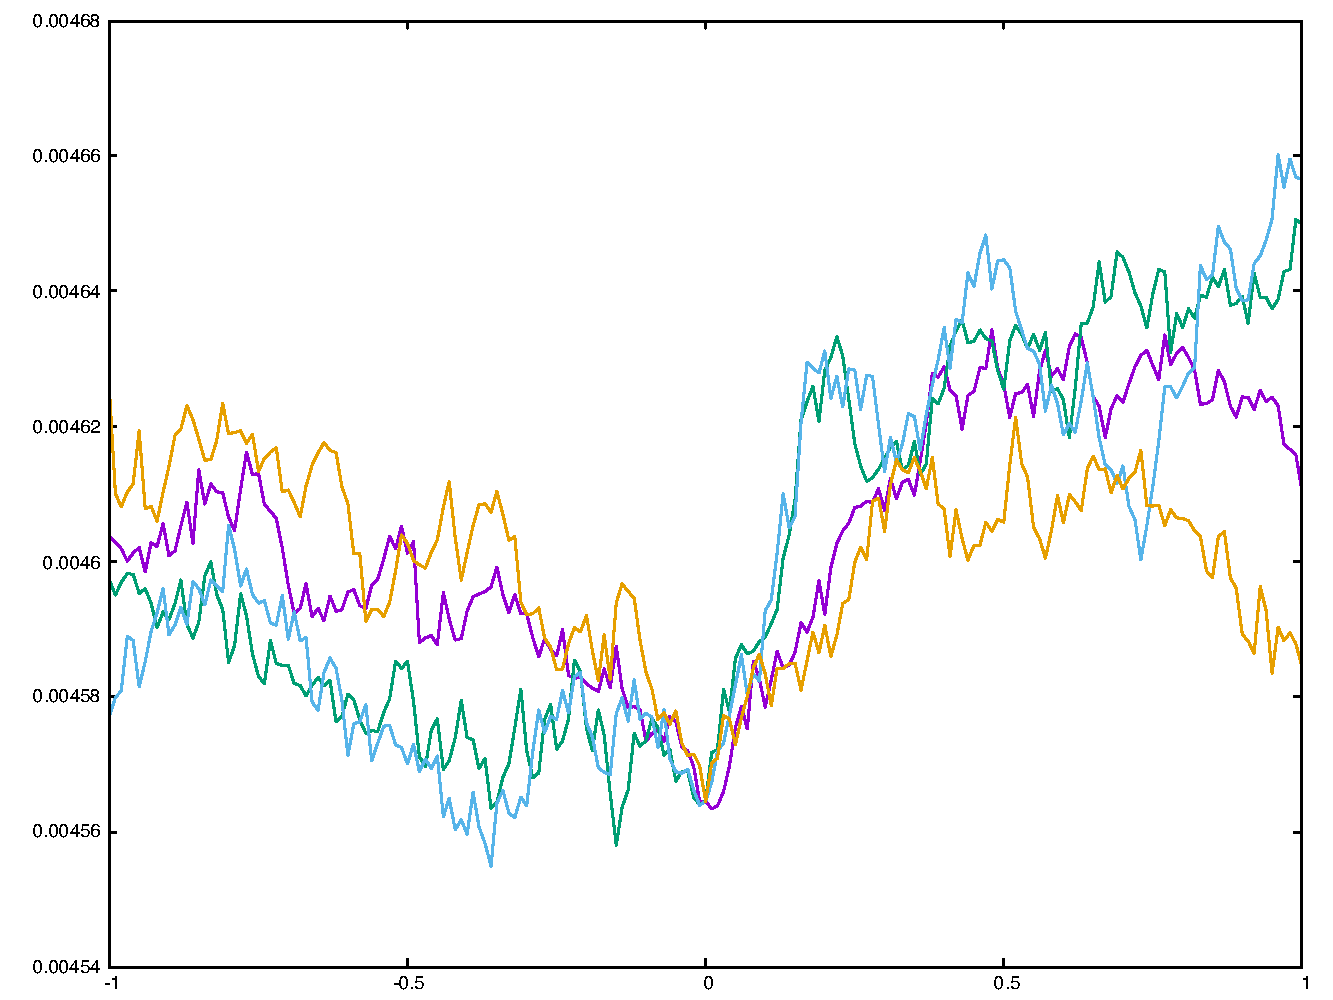
\includegraphics[width=\linewidth]{fig/ajherr/t3rr/c1.pdf}
	\caption{Centered on true transformation}
\end{subfigure}%
\begin{subfigure}{.49\textwidth}
	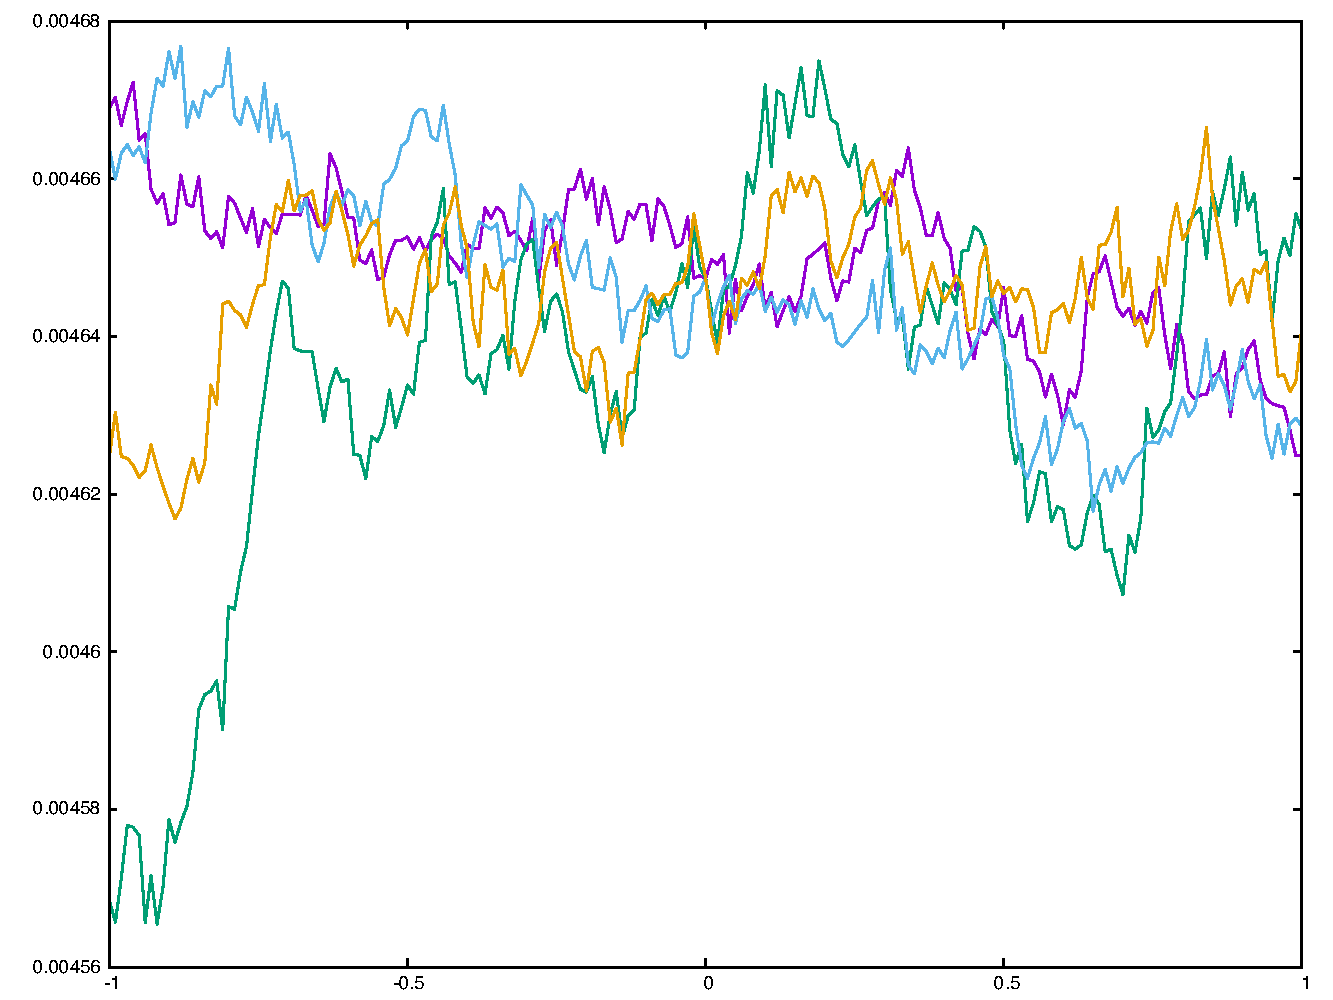
\includegraphics[width=\linewidth]{fig/ajherr/t3rr/c2.pdf}
	\caption{Centered on random transformation}
\end{subfigure}
\end{figure}

On the second plot, the cross sections in the rigid transformation space were instead chosen to intersect at another random transformation located near the true transformation $\matr{M}$. Here the curves still intersect, but no local minimum can be observed.

This result may have been by chance. However, it shows that the inflection points of the curves are not a side effect of the interpolation in the transformations space at $t = 0$. It is were so, it would also be visible on the second plot.

Because $P$ and $Q$ are point clouds generated from different projections of the relief model, they also have no coinciding points at the true transformation $\matr{M}$. So it seems that the \gls{arcdh} at the true transformation does not have special properties resulting from the experiment setup, that would explain this anomaly. Possibly $e_{r,\chi}$ is indeed an error metric that extracts additional information on the surface geometry from the point dispersion.

For the \gls{arcdh}, when $P$ and $Q$ are well aligned, more sample points $q \in Q$ get projected onto the correct locally planar surfaces of $P$, where they form a more uniformly distributed sample for measuring the closest point distances in the parallelogram lattices. This probably cannot be applied to real point scans either.


\section{Algorithm}
Putting everything together, the values $e_{\chi}$ and $e_{r,\chi}$ can be computed from the point clouds $P$ and $Q$ using the following algorithm. It is assumed that $P$ and $Q$ are already approximatively aligned.

$\matr{L}$ is the \emph{linear part} of the transformation which puts points $p \in P$ back into the coordinate system where the range image's camera is at origin. $p_l$ is the square width and height on the camera's image plane. $\alpha, \beta$ are the parameters for the obliqueness condition threshold of formula \ref{eq:pargrid_lmin_cond} from chapter \ref{ch:analysis_pc}. $\gamma$ is the maximal allowed angle between the normal vectors of corresponding points.

$c_{\text{max}}$ is the maximal allowed curvature measure, and $c(p)$ is the local curvature function defined in section \ref{sec:curvature} of the previous chapter. Here also its radius $r$ and its parameters $A$ and $D$ need to be fixed to some value.

$m \in \mathbb{N}$ is the number of bins in the histogram. The flag $\text{rej}$ indicates whether $e_{r,\chi}$ should be computed instead of $e_{\chi}$. It can be seen that there is no need to record all the correspondences in a list, and thus the spatial complexity is limited to the number of bins of the histogram.

\begin{figure}[H]
\begin{algorithmic}

\Function{RegistrationError}{$P, Q, \alpha, \beta, \gamma, c_{\text{max}}, m, \matr{L}, p_l, \text{rej}$}
	\State{$\text{ca} \gets \cos \alpha$}
	\Comment{Pre-calculate trigonometric function values for $\alpha$ and $\beta$}
	\State{$\text{tb} \gets \tan \beta$}
	\State{$\text{t1} \gets \tan (\frac{\pi}{4} - \beta)$}
	\State{$\text{t2} \gets \tan (\frac{\pi}{4} + \beta)$}
	
	\State{$\text{cc} \gets \cos \gamma$}
	\Comment{For normal compatibility test}
	
	\For{$i \in [0, m[$} \Comment{Initialize histogram}
		\State{$f[i] \gets 0$}
	\EndFor{}
	\State{$f_{\text{total}} \gets 0$}
	
	\ForAll{$(\vec{q}, \vec{n_q}) \in Q$}
		\Comment{Take coordinates $\vec{q}$ and normal vector $\vec{n_q}$ for each sample point}
		\State{$(\vec{p}, \vec{n_p}) \gets \text{closestPoint}(P, \vec{q})$}
		\Comment{Find closest model point $p \in P$}
		\State{$d \gets \| \vec{p} - \vec{q} \|$}
		\If{$(d > d_{\text{max}}) \vee (| \vec{n_p} \cdot \vec{n_q} | \leq \text{cc}) \vee (c(p) > c_{\text{max}})$}
			\Comment{If distance too large...}
			\State{\textbf{break}}
			\Comment{...normals incompatible or curvature too high, reject}
		\EndIf
		\State{$\vec{n} \gets \matr{L} \, \vec{n_p}$}
		
		\Comment{$n_p$ from point of view of the camera of $P$}
		\If{$|n_z| \leq \text{ca}$}
			\Comment{Check threshold condition for obliqueness}
			\State{$r \gets | \frac{n_x}{n_y} |$}
			\State{$r^{-1} \gets | \frac{n_y}{n_x} |$}
			\If{$(r < \text{tb}) \vee (r^{-1} < \text{tb}) \vee (\text{t1} < r) \vee (r < \text{t2})$}
				\State{\textbf{break}}
			\EndIf{}
		
			\If{rej}
				\State{$\vec{d} \gets \vec{q} - \vec{p}$}
				\Comment{When computing rejection error, project $q$ on $P$...}
				\State{$\vec{p}_{\text{proj}} \gets \vec{q} - (\vec{n_p} \cdot \vec{d}) \vec{n_p}$}
				\State{$d \gets \| \vec{p}_{\text{proj}} - \vec{p} \|$}
				\Comment{...and set $d$ to rejection distance}
			\EndIf{}
		
			\State{$l_{\text{min}} \gets p_l \, \sqrt{1 + \frac{\min \left\{
				n^2_x, \,
				n^2_y, \,
				1 + 2 \, n_x \, n_y, \,
				1 - 2 \, n_x \, n_y
			\right\} }{n^2_z}}$}
			\Comment{Compute $l_{\text{min}}$ and adjusted distance $a$}
			\State{$a \gets \frac{2 d}{l_{\text{min}}}$}
		
			\State{$i \gets \lfloor m \times a \rfloor$}
			\Comment{Select bin $i$ of histogram}
			\If{$i > m$}
				\State{\textbf{break}}
			\EndIf
		
			\State{$f[i] \gets f[i] + 1$}
			\Comment{Record value in histogram}
			\State{$f_{\text{total}} \gets f_{\text{total}} + 1$}
		\EndIf
	\EndFor
\algstore{errchi}
\end{algorithmic}
\end{figure}


\begin{figure}[H]
\begin{algorithmic}
\algrestore{errchi}
	\State{$\chi^2 \gets 0$}
	\Comment{Initialize chi-squared error $\chi^2$}
	\State{$w \gets \frac{1}{m}$} \Comment{Width of histogram bin}
	\State{$c \gets \frac{w}{2}$} \Comment{Center of current bin}
	\For{$i \in [0, m[$}
		\State{$o \gets \frac{f[i]}{f_{\text{total}}}$} \Comment{Normalized observed frequency}
		\State{$e \gets 2 w c$} \Comment{Normalized expected frequency}
		\State{$\chi^2 \gets \chi^2 + \frac{(o - e)^2}{e}$}
		\State{$c \gets c + w$}
	\EndFor
	
	\Return{$\chi^2$}
\EndFunction

\end{algorithmic}
\end{figure}



